\documentclass[]{acmtrans2m}
\usepackage{url}
\usepackage{graphicx}


\newtheorem{theorem}{Theorem}[section]
\newtheorem{conjecture}[theorem]{Conjecture}
\newtheorem{corollary}[theorem]{Corollary}
\newtheorem{proposition}[theorem]{Proposition}
\newtheorem{lemma}[theorem]{Lemma}
\newdef{definition}[theorem]{Definition}
\newdef{remark}[theorem]{Remark}

\newcommand{\firstrev}[1]{#1}
\newcommand{\comment}[1]{}

\title{Comparing Integer Data Structures for 32 and 64-bit Keys}

\author{
NICHOLAS NASH\footnote{Supported by Irish Research Council for Science, Engineering and Technology (IRCSET)} and DAVID GREGG\\
Trinity College Dublin
}

\category{E.1}{Data}{Data Structures}[Trees]
\terms{Algorithms, Experimentation, Measurement, Performance}
\keywords{Integer keys, Searching, Trees, Tries, Level compression}

\begin{abstract}
In this paper we experimentally compare a number of data structures operating over keys that are 32 and 64-bit integers.
We examine traditional comparison-based search trees as well as data structures that take advantage of the fact that the
keys are integers such as van Emde Boas trees and various trie-based data structures.
We propose a variant of a \textit{burst trie} that performs better in time than all the alternative data structures.
In addition, even for small sets of keys, this burst trie variant occupies less space than comparison-based data structures
such as red-black trees and $B$-trees.
Burst tries have previously been shown to provide a very efficient base for implementing cache efficient string sorting algorithms.
We find that with suitable engineering they also perform excellently as a dynamic ordered data structure operating over integer keys.
We provide experimental results when the data structures operate over uniform random data. We also present experimental results for other types of data, 
including data sets arising from \textit{Valgrind}, a widely used suite of tools for the dynamic
binary instrumentation of programs. 
\end{abstract}

\begin{document}

\maketitle

\begin{bottomstuff}
Corresponding author's address: Nicholas Nash, Department of Computer
Science, University of Dublin, Trinity College, Dublin 2, Ireland. \texttt{nashn@cs.tcd.ie}.
\end{bottomstuff}

\section{Introduction}

\subsection{Background and Motivation}

Maintaining a dynamic ordered data structure over a set of
ordered keys is a classic problem, and a variety of data
structures can be used to achieve $O(\log n)$ worst-case time
for insert, delete, successor, predecessor
and search operations when maintaining a set of $n$ keys. Examples
of such data structures include AVL trees \cite{Knuth98}, $B$-trees \cite{BayerMcCreight72,Knuth98} 
and red-black trees \cite{Cormen+01}. Red-black trees in particular see widespread use via
their GNU \textsl{C++} STL implementation \cite{Stroustrup97}.

Where the keys are known to be integers,
better asymptotic results can be obtained by data structures that do not rely solely on pair-wise key comparisons. For example,
the stratified trees of van Emde Boas \citeyear{vanEmdeBoas77} support all operations
in $O(\log w)$ worst-case time, when operating on $w$-bit keys, while
Willard's $q$-fast tries \citeyear{Willard84} support all operations in $O(\sqrt{w})$ 
worst-case time. 

Such data structures are attractive because of their superior
worst-case times compared to comparison-based data structures.
However, it is a significant challenge to construct implementations 
that reveal their better asymptotic performance, especially without occupying 
a large amount of extra space compared to comparison-based data structures.
For example, Dementiev \textit{et al.} \citeyear{Dementiev+04} provide a stratified tree implementation based 
on the variation described by Mehlhorn and N\"aher \citeyear{MehlhornNaher90}. While
they achieve superior performance in time against comparison-based data structures, their
data structure occupies more than twice as much space and is restricted to 32-bit keys.

In this paper we experimentally evaluate the performance of a variety of data structures when
their keys are either 32 or 64-bit integers. In particular we find that a carefully engineered
variant of a \textit{burst trie} \cite{Heinz+02} provides the best performance in time and
space all the alternative comparison-based data structures. The data structure we
describe is a bucketed trie with path compression and level compression \cite{AnderssonNilsson93}. 
To the best of our knowledge, the combination of level compression with bucketing in a trie has not
been studied experimentally in the past. In previous work \cite{NashGregg08} we described the
engineering of burst tries without the use of level compression. A key contribution of this work
is to demonstrate that level compression also results in a very efficient burst trie variant, while
using less space than our previously described variant, especially when the data structure contains
only a small set of keys.

We also emphasize that although we refer to the keys as integers, 
the keys may be any set of bit-strings all of some fixed length. Thus for example the keys
may be floating point numbers. Floating point numbers in particular can be dealt with very simply since their order
is preserved when their bit representation is interpreted lexicographically \cite{IEEE-754-2008}\footnote{Actually,
minor modifications are required to ensure this: the most significant bit is complemented for non-negative
floating numbers, all bits are for complemented negative floating point numbers.}.

\subsection{Related Work and Contributions}
\label{related_work}

In this paper we compare the performance of a carefully engineered variant of a burst trie in both time and space to
red-black trees and $B$-trees. Aside from these commonplace general purpose data structures, we also
experimentally examine the performance of two slightly more ad-hoc data structures \cite{Dementiev+04,KordaRaman99} 
that are tailored for the case of integers keys, and have been shown to perform well in practice. We briefly describe these
data structures in the remainder of this section.

Dementiev \textit{et al.} \citeyear{Dementiev+04} describe the engineering of a data structure based
on stratified trees \cite{vanEmdeBoas77} and demonstrate experimentally that it achieves superior performance to comparison-based data structures. 
We refer to their engineered data structure as an $S$-tree.
Although highly efficient in time, the $S$-tree is tailored around keys of 32-bits in length
and generalizing the data structure to 64-bit keys would not be feasible in practice because of
the large amount of space required to maintain efficiency. Indeed, even for 32-bit keys the data structure
requires more than twice as much space as a typical balanced search tree.

Korda and Raman \citeyear{KordaRaman99} describe a data structure similar to a $q$-fast
trie \cite{Willard84} and experimentally show that it offers performance superior to comparison-based data structures.
Unlike the $S$-tree data structure engineered by Dementiev \textit{et al.} this data structure is not restricted to 
32-bit keys and requires less space in practice. We now briefly describe the features of Korda and Raman's data structure
relevant to our discussion. We refer to their data structure as a $Q$-trie.
A $Q$-trie consists of a path compressed trie containing a set of \textit{representative
keys}, $K_1 < K_2 < \cdots < K_m$. Associated with each representative key $K_i$ is a bucket data structure $B_i$
containing the set of keys $\lbrace k \in S : K_i \leq k < K_{i + 1} \rbrace$ for $i < m$, and
$\lbrace k \in S : k \geq K_m \rbrace$ for $i = m$, where $S$ is the entire set of keys in the data structure.

Each bucket contains between $1$ and $b - 1$ keys. When a new key is inserted into the data structure the compressed
trie is first searched for its predecessor key, giving a representative key $K_i$. If the associated bucket $B_i$ already
contains $b - 1$ keys, a new representative key is added to the compressed trie that partitions the bucket into
two new buckets containing $b/2$ keys each. Deletions operate in a similar manner to insertions, except that when two adjacent
buckets $B_i$ and $B_{i + 1}$ contain fewer than $b/2$ keys in total the keys of $B_{i + 1}$ are inserted
into $B_i$ and $K_{i + 1}$ is deleted from the trie. A search in the data structure is accomplished by a predecessor query in the 
compressed trie, followed by a search in the relevant bucket data structure.

There are many other non-comparison-based data structures in addition to the two just mentioned, both practical and theoretical. 
Two practical examples are the cache-friendly tries of Achyra \textit{et al.} \cite{Acharya+99} and the dictionaries described and experimentally
analyzed by Dietzfelbinger \textit{et al.} \citeyear{Dietzfelbinger+94,Dietzfelbinger+08}. However, we believe these
data structures are either less efficient or less general than the two data structures described above. 
For example, the data structure described by Dietzfelbinger \textit{et al.} is less general and does not efficiently support predecessor or successor
operations. Moreover, the tries of Achyra \textit{et al.} appear
efficient, but require knowledge of cache parameters and focus only on trie search. It is not clear how operations 
like predecessor and successor could be efficiently implemented, since hash tables are used inside the trie nodes.

The contribution of our experimental study is to show that a carefully engineered data structure based on the burst
trie described by Heinz \textit{et al.} \cite{Heinz+02} performs better than both the $S$-tree and $Q$-trie data structures
described above, as well as the traditional comparison-based data structures.

The work of 
Heinz \textit{et al.} focuses on the problem of \textit{vocabulary accumulation}, where the keys are variable length strings.
The only operations performed are insert and search, with a final in-order traversal of the burst trie.
In contrast, we consider the case of integer keys with all the operations usually associated with a dynamic
ordered data structure.

The contributions of our work are as follows:

\begin{itemize}
\item We provide a thorough experimental comparison of dynamic data structures over 32 and 64-bit integer keys.
      We provide time and space measurements over random data as well over other data sets, including those that occur in Valgrind, a
      notable application of such data structures.

\item We show that burst tries extend efficiently to a dynamic ordered data structure, showing how the operations usually associated
      with such data structures can be implemented efficiently through careful engineering.

\item We show that the data structure is more efficient in time than the best previous data structures that have been 
      engineered for the case of integer keys. Building on previous work \cite{NashGregg08}, we also show that, through the use of
      level compression, for even small numbers of keys the data structure requires less space than even space efficient implementations of comparison-based
      search trees. 
\end{itemize}

\begin{figure}[t]
\center
\begin{tabular}{cc}
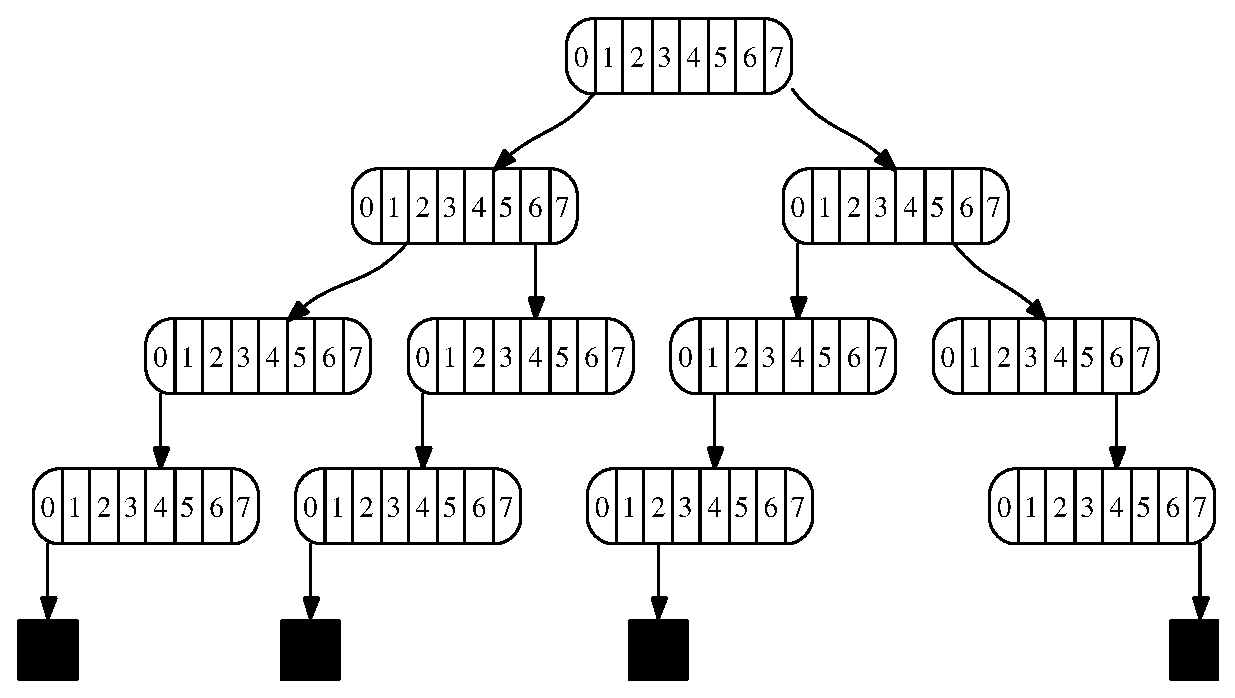
\includegraphics[width=0.5\textwidth]{figs/simple_trie.eps} & 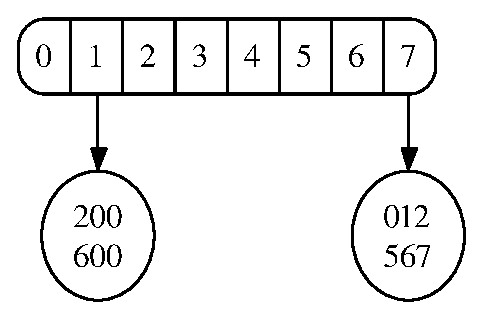
\includegraphics[width=0.3\textwidth]{figs/trie1.eps}\\
(a) & (b)\\
\end{tabular}
\caption{(a) Shows a trie holding the keys 1200, 1600, 7012
and 7567. The leaves of the trie (black squares) hold the satellite
data associated with the keys. A corresponding burst trie, with bucket capacity 2, is shown in (b).}
\label{simple_trie}
\end{figure}

\section{Background}
\label{background}

In this section we provide the definition of a burst trie and some
basic background information regarding the data structure.

\begin{definition}
A string $w$ is the $v$-suffix of a string $u$ if $u = vw$.
\end{definition}

\begin{definition}
A \textit{burst trie} with bucket capacity $c$ containing $n$ keys is a tree with the following properties:
\begin{enumerate}
    \item If $n = 0$, the burst trie is empty.
    \item If $n > c$, the burst trie consists of an internal node with $2^i$ children, $i \geq 1$. 
          For each binary string $x$ of length $i$, there is a child burst trie containing all the $x$-suffixes of
          the keys.
    \item If $n \leq c$, the burst trie is a bucket data structure containing the $n$ keys and their associated values.
\end{enumerate}
\end{definition}

Figure \ref{simple_trie}(a) shows an example of a trie while Figure \ref{simple_trie}(b)
shows a burst trie corresponding to it. Although we refer to what has just been described as a burst trie, using some kind of bucketing
in a trie is an old technique. Sussenguth \citeyear{Sussenguth63} provides an early suggestion of the technique, 
while Knuth analyses bucketed tries \citeyear{Knuth98}. In addition, Knessl and Szpankowski \citeyear{KnesslSzpankowski00a,KnesslSzpankowski00b} 
analyse what they refer to as $b$-tries --- tries in which leaf nodes hold up to $b$ keys. 

We use the term burst trie of Heinz \textit{et al.} \citeyear{Heinz+02} because their work was the first to
provide a large scale investigation of alternative bucket data structures, the time and space trade-offs
in practice resulting from bucketing, and the \textit{bursting} of bucket data structures during insertions,
which we describe below.

Searching in a burst trie is similar to searching in a conventional trie.
The digits of the key are used to determine a path in the trie that either terminates
with a \textsc{nil} pointer, in which case the search terminates unsuccessfully, or a bucket is found.
In the latter case, the search finishes by searching the bucket data structure for the key
suffix.

Insertion of a key into a burst trie is also straightforward. The digits of the key are used to locate
a bucket where the key suffix should be stored. If no such bucket exists, one is created. On the other
hand, if a bucket is found and it contains fewer than $c$ keys it need not be burst and the key suffix
is simply added to that bucket. Otherwise, if the bucket already contains $c$ keys, it is burst. This
involves replacing the bucket with a trie node and distributing the keys suffixes of this bucket into new buckets
descending from this new trie node. Figure \ref{burst_fig}(a) shows an example of a burst operation
occuring on the burst trie of Figure \ref{simple_trie}(b). It is possible that all keys from the
burst bucket belong in the same bucket in the newly created node. In this case, the bursting process is repeated.

Deleting a key $k$ from a burst trie is performed by first searching for the bucket where $k$ is stored, as described
above. If there is no such bucket, no deletion need occur. Otherwise, $k$ is deleted from some bucket $b$ at 
a node $x$. If $b$ is then empty, it is deleted from $x$. If $x$ then has only \textsc{nil} child and bucket pointers
$x$ is deleted from the trie. This step is repeated, traversing the path from $x$ to the root of the trie
deleting ancestors encountered with only \textsc{nil} child or bucket pointers. 
The traversal terminates when either a node with a non-nil pointer is encountered, or the root of the trie
is reached.

\begin{figure}%[t]
\center
\begin{tabular}{cc}
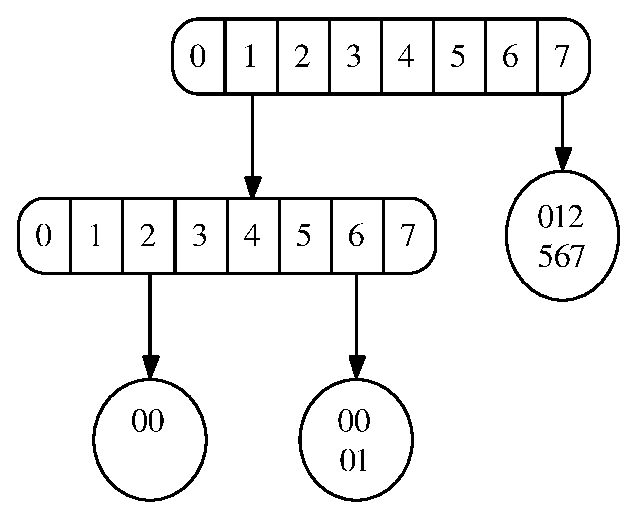
\includegraphics[width=0.35\textwidth]{figs/trie2.eps} & \includegraphics[width=0.45\textwidth]{figs/or_tree.eps}\\
(a) & (b)\\
\end{tabular}
\caption{(a) Shows the burst trie of Figure \ref{simple_trie}(b) after inserting the key 1601.
Assuming the buckets can hold at most two key suffixes, inserting the key 1601 causes the left
bucket shown in Figure \ref{simple_trie}(b) to burst. In (b) an OR-tree is shown, a possible
in-node data structure for implementing a burst trie.}
\label{burst_fig}
\end{figure}

\section{Engineering Burst Tries}

Although the burst trie data structure described in the Section \ref{background} leads to a highly efficient
data structure, especially for strings, as shown by Heinz \textit{et al.} \cite{Heinz+02}, 
care must be taken when engineering it for the case of an ordered data structure for integer keys.
Our variant of a burst trie makes use of three data structures for which we consider the engineering concerns:
$(1)$ The trie data structure itself. We describe the use of a trie making use of level and
path compression. We note that the combination of level compression and bucketing in tries has not been examined experimentally
in the past. $(2)$ The bucket data structures at the leaves of the trie, and $(3)$ the data structures 
inside the nodes of the burst trie. We describe the alternatives for this latter data structure in the next section.

\subsection{In-Node Data Structures}
\label{in_node_structs}

Given a node $x$ in a trie-based data structure with branching factor $b$, and an index $i$, 
$0 \leq i < b$, it is often necessary to find $\mbox{\textsc{Succ}}(i)$, that is, the smallest $j > i$ such that 
$x\left[j\right] \neq \mbox{\textsc{nil}}$. This is the bucket or child node pointer directly
following $x\left[i\right]$. It is also often required to find $\mbox{\textsc{Pred}}(i)$, 
the largest $j < i$ such that $x\left[j\right] \neq \mbox{\textsc{nil}}$. 
These operations upon nodes are required, for example to support queries on the trie involving
in-order iteration over its keys. We elaborate on the precise use of these operations in Section \ref{operations}.

Many data structures can be used to support these predecessor and successor operations on the trie node
\cite{Demaine03}. We experimented with several in-node data structures for our burst trie variant.
The simplest 
data structure supporting these predecessor and successor operations is
just a linear search over a bit-vector.
This data structure requires only $O(1)$ time when a new bucket or child is added or removed
from the node, however, $\mbox{\textsc{Pred}}$ and $\mbox{\textsc{Succ}}$ are inefficient, requiring 
$O(b)$ time. 

An alternative in-node data structure is an OR-tree. Figure \ref{burst_fig}(b) shows an
example of this data structure. A breadth-first traversal of an OR-tree can be laid out in an array inside each node, 
requiring an additional $O(b)$ space compared to a simple bit-vector approach. However, an OR-tree offers
all operations in $O(\lg b)$ time.

Another simple solution is to implement $\mbox{\textsc{Pred}}$ and $\mbox{\textsc{Succ}}$ 
using $\lceil\sqrt{b}\rceil$ counters. Where the $i^{th}$ counter, $0 \leq i < \lceil \sqrt{b} \rceil$ 
holds a count of the non-zero bits in the range 
$[i\lceil \sqrt{b} \rceil, i\lceil\sqrt{b}\rceil + \lceil\sqrt{b}\rceil - 1]$
(except perhaps for the last counter, which covers the range $[b - \lceil\sqrt{b}\rceil, b - 1]$).
This data structure allows insertions and deletions in $O(1)$ time and supports 
$\mbox{\textsc{Pred}}$ and $\mbox{\textsc{Succ}}$ in $O(\sqrt{b})$ time, requiring at most $\lceil\sqrt{b}\rceil$
counters to be examined followed by at most $\lceil\sqrt{b}\rceil$ bits.

Of course, for large enough inputs the OR-tree will out-perform the counter search, because it executes asymptotically
fewer instructions. However, even for the largest experiments we conducted in 
this paper (see Section \ref{exp_comparison}), which include data sets of $2^{27} \approx 1.3 \times 10^7$ keys, the 
branching factor of any node in the burst trie did not exceed $2^{20}$. 
Moreover, it is clear that due to its breadth-first layout, the spatial locality of the OR-tree is worse than 
that of the counter search. The OR-tree is also likely to incur more branch mispredictions, since intuitively
one expects that an algorithm executing an asymptotically smaller number of branches extracts more information from
each branch, thus making each branch less predictable. 
The spatial locality of the OR-tree can be improved by avoiding the use of the breadth-first layout, instead
a cache oblivious layout can be used \cite{Bender+00,Brodal+02}.

Figure \ref{node_structs_plots} shows experimental measurements for the OR-tree in breadth-first and cache oblivious layouts, and the counter search
as the size of the bit-vector increases. The bit-vector in this case consists of all zeros
except that its right-most bit is set to a one. The searching operation here is to find the successor of the left-most
bit in the bit-vector. Figure \ref{node_structs_plots}(a) shows the cycles (i.e. time) per search operation. 
At the smaller input sizes, $b < 2^{13}$, the counter search is a maximum of approximately 30\% faster than the breadth-first
layout OR-tree (although this is not easily visible in Figure \ref{node_structs_plots}(a)). We note that
the OR-tree cleary out-performs the counter search from around $b = 2^{13}$ onwards.  This is due to the rapidly increasing
instruction count of the counter search compared to the OR-tree, shown in Figure \ref{node_structs_plots}(b). The 
smaller number of cache misses and branch mispredictions incurred by the counter search, shown in Figure \ref{node_structs_plots}(c) and (d) respectively are not 
enough to compensate for this difference. For the range of input sizes considered here, the improved spatial locality of the cache oblivious layout OR-tree
is not enough to compensate for the increase in instruction count and branch mispredictions that the more complicated 
indexing of the cache oblivious layout causes. It should be noted that the cache misses shown in Figure \ref{node_structs_plots} are level 1 misses, and are
less expensive than the usually considered level 2 misses.

\comment{
A compromise between the instruction counts, branch prediction characteristics and data cache misses of the counter
search and the OR-tree can be obtained by dividing the bit vector into chunks of size $B$. Counter searches are used
in these chunks, and an OR-tree with $b/B$ leaves is formed over the chunks. 
As expected, the hybrid searching technique has an instruction count, cache miss rate and branch misprediction rate between that of the 
counter search and the OR-tree. However, as Figure \ref{node_structs_plots}(a) shows, this trade-off in constant factors does not result
}

In our burst trie variant, we have chosen to use the OR-tree as the in-node data structure. This engineering decision
is based on the data just presented. It should be noted that the experiments above consider the case where the trie nodes are
very sparse, and the bits are not distributed uniformly. If one expects denser nodes and the burst trie to contain data with a high degree of randomness 
then the counter search is preferable. For example, note that if a bit-vector of any number of bits has only $0.1\%$ non-zero bits and these are uniformly distributed then successor queries 
on the in-node structure can be regarded as operating on bit-vectors of 1000 bits long on average, which is well within the region for which the
counter search performs comparatively well (see Figure \ref{node_structs_plots}(a)), and moreover it requires only $O(\sqrt{b})$ rather than $O(b)$ extra space. 

\begin{figure}%[t]
\center
\begin{tabular}{cc}
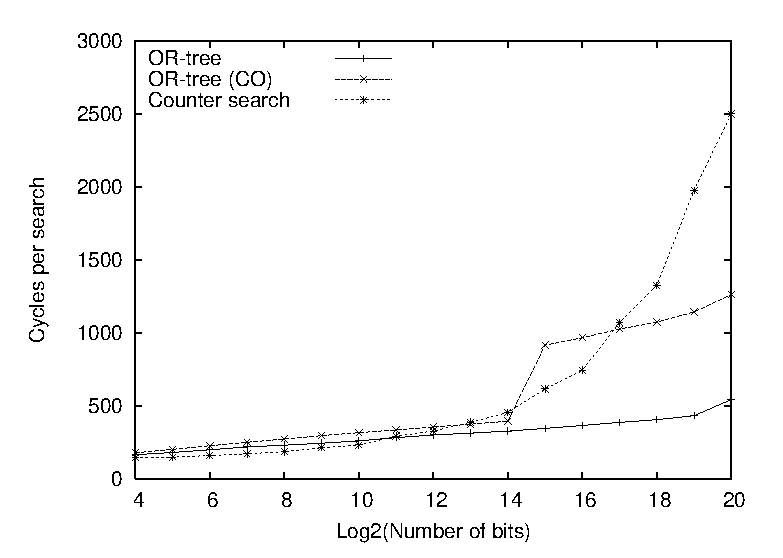
\includegraphics[width=0.485\textwidth]{plots/nstructs_cyc.eps} & 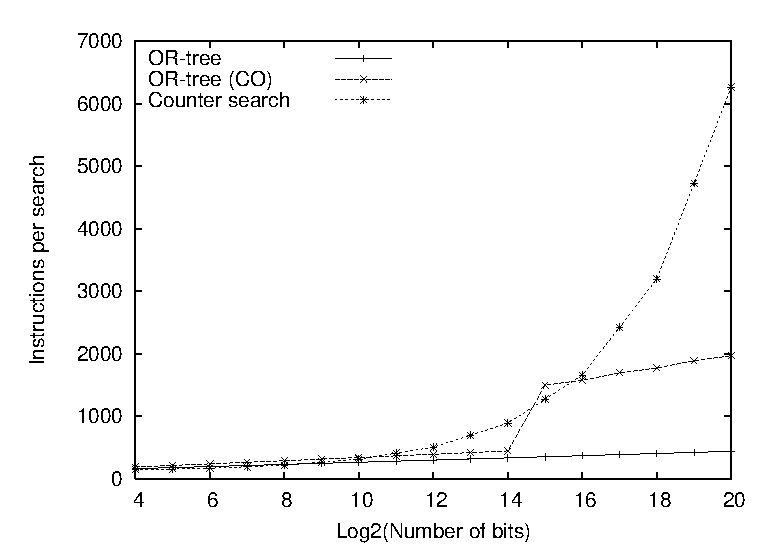
\includegraphics[width=0.485\textwidth]{plots/nstructs_ins.eps}\\
(a) & (b)\\
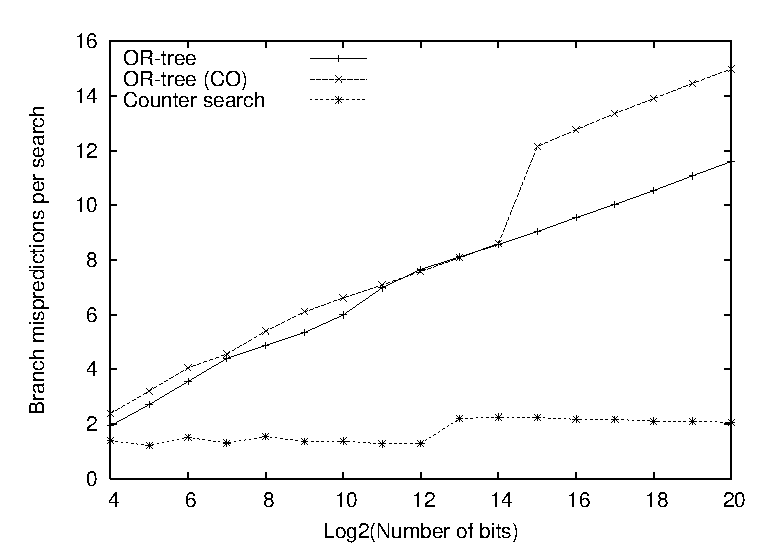
\includegraphics[width=0.485\textwidth]{plots/nstructs_brmsp.eps} & 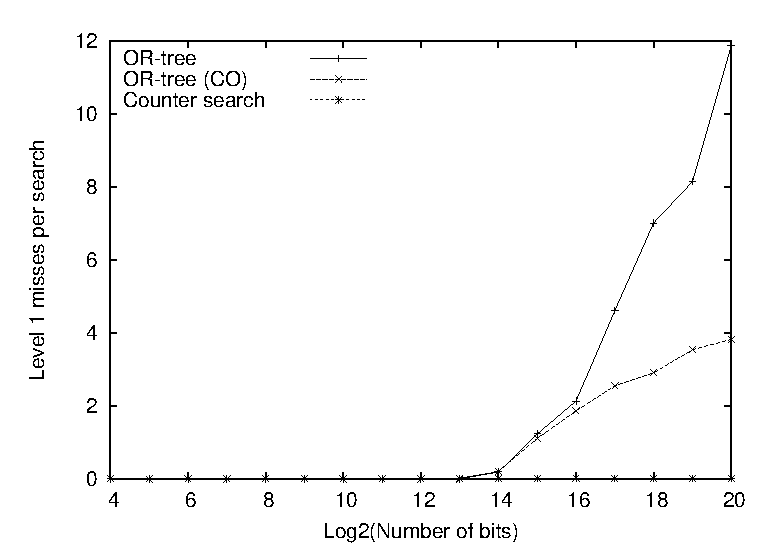
\includegraphics[width=0.485\textwidth]{plots/nstructs_l1dcm.eps}\\
(c) & (d)\\
\end{tabular}
\caption{This figure shows a comparison of the in-node data structures described in Section \ref{in_node_structs}. The results are averaged
over several thousand successor search operations on a sparse bit-vector, and were gathered using PAPI [Dongarra et al. 2003] on an Intel Core 2
2.13GHz, having a 32KB level 1 data cache. All of the data structures fit within the level 1 data cache. We note the reduced branch mispredictions
of the counter search, shown in (c) and its better spatial locality shown in (d), are not enough to compensate for its larger instruction count
compared to the OR-tree, shown in (b). As a result, except for very small inputs, the OR-tree performs best, as is shown in (a). 
The cache oblivious OR-tree is labelled ``OR-tree (CO)''. Due to the extra expense of computing the cache oblivious
indexing for this data structure, its performance is worse than the standard OR-tree, despite its better spatial locality, visible in (d). 
The transition points visible in the cache oblivious OR-tree's 
performance at $2^{15}$ bits are a result of that fact that at $2^{15}$ bits indexing reverts to breadth-first layout (without this reversion,
the overhead of its cache oblivious indexing is even higher).}
\label{node_structs_plots}
\end{figure}


\subsection{Bucket Data Structures}
\label{bucket_structs}

The choice of data structure used for the buckets of a burst trie is critical in achieving
good performance. Heinz \textit{et al.} \cite{Heinz+02} concluded that unbalanced binary
search trees holding at most 35 strings offered the best performance as a bucket
data structure. They also experimented with linked lists and splay trees \cite{SleatorTarjan85}.
Since the maximum number of keys stored in each bucket is modest (at most 35), a simple
bucket data structure, even with bad asymptotic behaviour, may perform well. 
In related work, unsorted arrays of strings
have been used as bucket data structures for burst tries as a basis for the \textit{burstsort}
algorithm \cite{SinhaWirth08,Sinha+06,SinhaZobel05,SinhaZobel04,Sinha04}, which is a cache-efficient radix sorting algorithm.

We experimented with balanced binary trees as well as with unsorted arrays and sorted arrays.
Over all, we found the arrays are far more efficient in practice than the search trees. 
It is likely that the arrays incur far fewer cache misses than the search trees. 

If unsorted arrays of $c$ elements are used as the bucket data structures, searching in a bucket takes $O(c)$ time.
Insertion also requires $O(c)$ time, because each key to be inserted must be searched for in the bucket
before it can be inserted in order to avoid duplication. If sorted arrays are used, searching in a bucket takes $O(\lg c)$ time, while insertion
takes $O(c)$ time. In practice, the insertion into a sorted array is more expensive than the
insertion into an unsorted array. This is because in unsorted arrays the elements need simply be scanned to
check for the presence of the key to be inserted. In the sorted case the elements of the array must be rearranged
to maintain sorted order. However, the logarithmic search time in sorted buckets gives much improved search
times in practice. Since in many applications, searching is the most frequent operation executed on a data structure
we have chosen the sorted arrays over the unsorted arrays. In addition, predecessor and successor operations are
less efficiently supported by unsorted arrays.

In contrast to the array buckets of the burstsort algorithm, our buckets are sorted holding at most 128 keys.
This is in contrast to the bucket sizes used in burstsort, where the buckets are allowed to grow until they reach the size of the processor's 2nd level cache
which can be several megabytes in size. The buckets are implemented as growable
arrays, and an insertion involves possibly doubling the size of the bucket followed by a linear scan
to find the correct position for the key to be inserted. 

As mentioned above, often the most frequent operation executed on a data structure is a search, and so searching buckets in
particular should be efficient. We use a binary search that switches to a linear search when the number
of keys which remain to be searched falls below a certain threshold. We found a threshold of between
16 and 32 keys gave a performance improvement over a simple binary search. Our burst trie implementation
is designed to provide a mapping from a key to the satellite data associated with that key, which we 
refer to as the \textit{value} for the key.  
To improve the spatial locality of searches the keys and values of a bucket should not be interleaved.
Rather, all the keys should be stored sequentially, 
followed by all the values of that bucket. This ensures searching for a key makes better utilization of 
the processor's cache lines.

If the maximum bucket capacity is $c$, it takes $O(c)$ time to insert into
a bucket and $O(\lg c)$ time to search in a bucket. Finally, since bursting a bucket (see Section \ref{background}) 
just involves splitting the sorted sequence of keys it contains into a number of other sorted
sequences, bursting a bucket also takes $O(c)$ time.

\subsection{Level and Path Compressed Tries}
\label{level_path_comp}

\begin{figure}%[t]
\center
\begin{tabular}{cc}
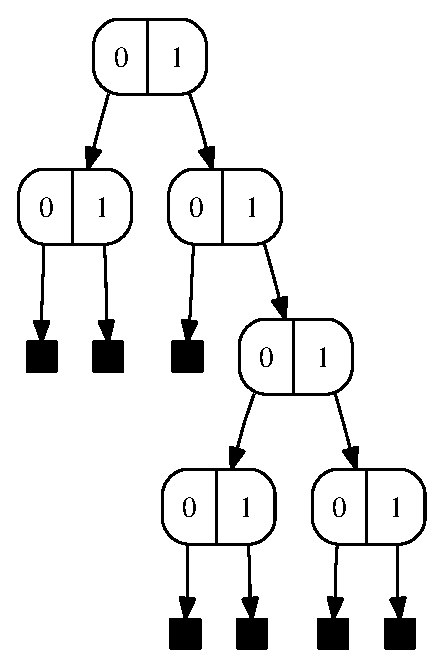
\includegraphics[width=0.3\textwidth]{figs/binary_trie.eps} & 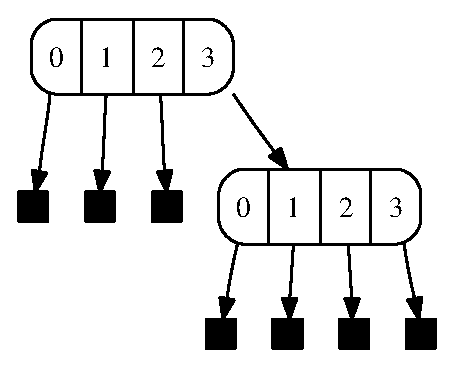
\includegraphics[width=0.35\textwidth]{figs/lc_trie.eps}\\
(a) & (b)\\
\end{tabular}
\caption{(a) Shows a binary trie, while (b) shows a level compressed trie. The level compressed trie in (b) is obtained
from (a) by replacing the top-most $i$ complete levels of the trie with a single node of branching factor $2^i$, and then
repeating the process on the children.}
\label{lctrie_fig}
\end{figure}

The burst trie defined in Section \ref{background} uses a simple trie to search for
the bucket in which a key resides. In this paper we investigate experimentally the
case where the burst trie is both level and path compressed. Level compression
was proposed by Anderson and Nilsson \citeyear{AnderssonNilsson93} (see also Nilsson \citeyear{Nilsson96}). 
Dynamic level and path compressed tries, or
$LPC$-tries were investigated experimentally by Nilsson and Tikkanen \citeyear{NilssonTikkanen02}. 
However, they concluded level compression gave rise to tries that offered slower insertions
and deletions than comparison-based structures, while offering faster search operations.
Moreover, their $LPC$-tries occupy a similar amount of space to comparison-based search
trees. In contrast, the bucketed variations we describe in general provide all operations
more efficiently than comparison-based search trees, while also occupying signficantly less
space.

We next give the definition of a path compressed burst trie ($PCB$-trie) and then of a level and path 
compressed burst trie ($LPCB$-trie), slightly amending the definitions of an $LPC$-trie given
by Nilsson and Tikkanen \citeyear{NilssonTikkanen02}.

\begin{definition}
A \textit{path compressed burst trie} or \textit{$PCB$-trie} with bucket capacity $c$ containing $n$ keys is a tree 
with the following properties:
\begin{enumerate}
    \item If $n = 0$, the $PCB$-trie is empty.
    \item If $n > c$, the $PCB$-trie consists of an internal node with $2^i$ children, $i \geq 1$,
          and a binary string $x$. The string $x$ is the longest common prefix  
          of all the keys stored in the $PCB$-trie. For each binary string $y$ of length $i$, 
          there is a child trie containing all the $xy$-suffixes of the keys.
    \item If $n \leq c$, the $PCB$-trie is a bucket data structure containing the $n$ keys and their associated values.
\end{enumerate}
\end{definition}

\begin{definition}
A \textit{level and path compressed burst trie} or \textit{$LPCB$-trie}, with bucket capcity $c$, is a tree with the following properties: 
\begin{enumerate}
    \item The root is a $PCB$-trie with bucket capacity $c$ having $2^i$ children, where $i \geq 1$ is chosen as large as possible such
          that the root has no empty child tries.
    \item Each child trie of the root is an $LPCB$-trie.
\end{enumerate}
\end{definition}

\noindent
Figure \ref{lctrie_fig} shows a simple example illustrating the idea of level compression in a trie.

Maintaining level compression dynamically is achieved through \textit{doubling} and \textit{halving} of trie nodes.
Doubling a trie node of branching factor yields a new trie node having twice the number of children
of the original node, with the children shifted up (at most) one level of the trie accordingly. Similarly, halving a trie node reduces
its branching factor by half, shifting down its children through the introduction of new binary nodes where necessary. For full
details of doubling and halving, the reader is referred to the description of Nilsson and Tikkanen \citeyear{NilssonTikkanen02}.

The level compression defined for the $LPCB$-trie is what Nilsson and Tikkanen \citeyear{NilssonTikkanen02} refer to as \textit{perfect}.
In a dynamic setting, a more relaxed approach to level compression results in a more robust data structure.
Nilsson and Tikkanen point out that maintaining perfect level compression dynamically can cause a simple sequences of alternating insertions and deletions to cause 
computationally expensive restructurings of the trie. Instead it is desirable to associate two parameters $\alpha, \beta \in [0, 1], \alpha < \beta$ with the trie. 
A node of branching factor $2^i$ is halved if the number of empty sub-tries is greater than or equal to $\lfloor \alpha 2^i \rfloor $.
A node is doubled if the result is a new node of branching factor $2^i$, of which at least $\lfloor \beta 2^i \rfloor$ of its subtries are non-empty.
In all experiments in this paper, we have used $\alpha = 1/4$ and $\beta = 3/4$. Surprisingly, Janson and Szpankowski \citeyear{JansonSzpankowski07} have shown that using this so-called
\textit{partial fill-up} in a level compressed trie results in a \textit{smaller} constant factor in the leading term of asymptotic search times in level compressed tries in the Bernoulli model. 

The combination of level and path compression is straightforward, all the trie-based structures we present results for in this paper
are both level and path compressed. In the experiments presented here the minimum branching factor of any node in the level
compressed trie structures is 16. We found this to offer a reasonable trade-off between time and space in the trie. Allowing
nodes with very small branching factors can lead to large amounts of memory allocation, note also that a substantial proportion of
the storage of smaller nodes is simply overhead from the memory allocations required for the node and its internal structures.

We conducted a simple experiment to compare the performance of burst tries without either level or path compression, with level compression only, with path compression only,
and with both level and path compression. A description of the experimental setup used to gather these results can be found in Section \ref{exp_comparison}. Further details of how the
trie structures are implemented can be found in Section \ref{operations}.

Figure \ref{burst_trie_comparison_fig}(a) shows the time per \textit{locate} operation on burst tries using the bucket and node structures described in the preceding two sections,
where the trie structure used to index the buckets is varied. The locate operation returns the value associated with the largest key less than or equal to the key provided to it.
We have chosen this operation because it is more general than can be answered efficiently with a hash table. 
The keys inserted into and searched for in the tries are uniform random 32-bit keys.

As Figure \ref{burst_trie_comparison_fig}(a) shows, the burst tries making use of level compression (the $LCB$-trie and $LPCB$-trie) are slightly more efficient than those that do not. 
Note that since the data inserted into the tries is uniformly distributed the path compression has little influence on the performance of the data structures. 

Figure \ref{burst_trie_comparison_fig}(b)
shows the space required by the data structures as the number of inserted keys increases. For small sets of keys, the $WB$-trie and $PCB$-trie require much more memory than
the two level compressed tries. The $WB$-trie is a simple burst trie (without level or path compression) but with a wide root node, of branching factor $2^{16}$. The $PCB$-trie
is a burst trie with path compression and also having a root node of branching factor $2^{16}$. In the $WB$-trie and $PCB$-trie all children nodes have branching factor $2^6$.
These parameters were chosen because they appeared to offer a favourable trade-off between time and space on this data. Finally the $TB$-trie is a burst trie without level
or path compression where the root node does not have a large branching factor. In particular, every node has branching factor $2^8$. As Figure \ref{burst_trie_comparison_fig}(b), the $TB$-trie is also much
less efficient in space than the two level compressed tries.

As a result of these experiments we have chosen to use the $LPCB$-trie in our experimental comparison with other integer data structures.
The results show that level compression appears to result in trie structures with more efficient search operations than those without it. More importantly, the level compressed
tries require substantially less space. 

\begin{figure}
\center
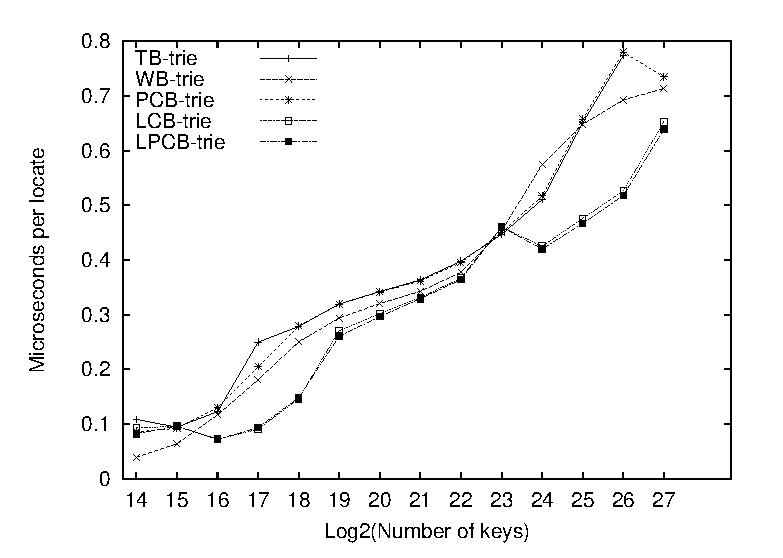
\includegraphics[width=0.8\textwidth]{plots/burst_irandom_time_knuth.eps}\\
(a)\\
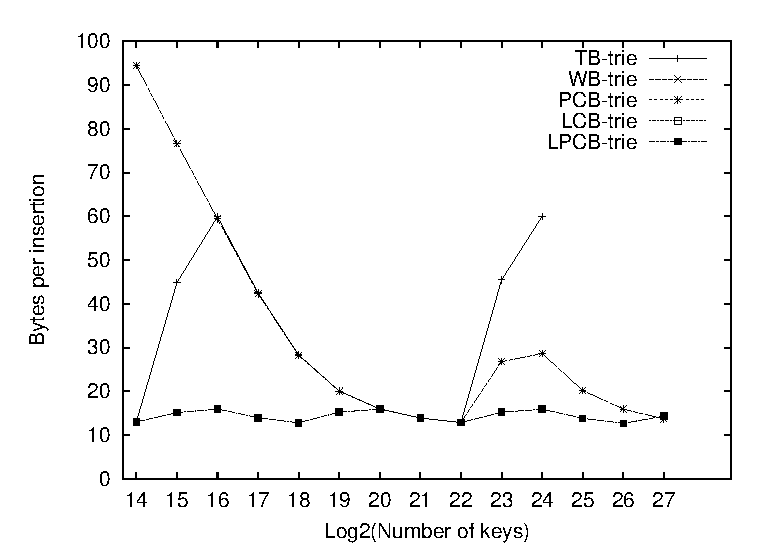
\includegraphics[width=0.8\textwidth]{plots/burst_irandom_mem_knuth.eps}\\
(b)
\caption{(a) Shows the average time required by the trie structures to perform a \textit{locate} operation for a uniform random 32-bit key
as the number of keys inserted into the data structure increases. 
The burst trie without either level or path compression and with a wide root is labelled ``$WB$-trie''. 
The burst trie without either level or path compression and also without a wide root is labelled ``$TB$-trie''.
The burst trie with path compression only is labelled ``$PCB$-trie''. The burst trie with level compression only is labelled ``$LCB$-trie''. Finally the burst trie with both level
and path compression is labelled ``$LPCB$-trie''. (b) Shows the memory required by the data structures.
Due to the slight overhead of measuring the memory consumed by the data structures we were unable to
measure the memory used by the $TB$-trie for data sets of $2^{25}$ random key insertions or higher.
Since path compression has little effect on this uniform random data, the memory consumption of the $WB$-trie and $PCB$-trie is essentially identical. Also, the memory consumption of the $LCB$-trie and $LPCB$-trie is almost identical
for the same reason. These results are discussed in Section \ref{level_path_comp}.}
\label{burst_trie_comparison_fig}
\end{figure}


\subsection{Operations}
\label{operations}

The preceding sections have described the data structures required for efficiently extending burst tries to 
an ordered data structure. We now show how these data structures can be used efficiently to provide a 
burst trie with all the usual operations associated with a dynamic ordered data structure. 
Note that in order that predecessor and successor operations are supported efficiently, it is wise to
maintain the leaves of the burst trie (i.e. the buckets) in order in a doubly linked list.
The operations described below are for a $LPCB$-trie with maximum branching factor $b$ and bucket capacity $c$. Recall
that we use an OR-tree as the in-node structure for the trie nodes, and growable sorted arrays as buckets in the trie.
We denote the maximum height of the trie as $h$, the value of which is determined by the number of bits in the keys
and the minimum branching factor allowed for nodes in the trie. The final two parameters associated with the $LPCB$-trie
are $\alpha$ and $\beta$, the ratios of empty to non-empty children that cause doubling and halving of
trie nodes, respectively.

\textbf{Locate.} We first describe the \textit{locate} operation, which finds the value associated  
with the largest key less than or equal to a supplied key $k$ (or \textsc{nil} if there is no such key).
Assuming the path in the burst trie determined by $k$ leads to a bucket, then that bucket is searched for
the smallest key suffix greater than or equal to $k$'s suffix, and its corresponding value is returned. If $k$ is not
found in this bucket, the result is the largest key in the bucket immediately before it in the linked list of buckets, which
can be found in constant time.
In this case, the locate operation takes $O(h + \lg c)$ time. In the case where $k$ does not lead to a bucket, the in-node data structure can be
used to find a bucket requiring $O(h + \lg b)$ time, thus \textit{locate} requires $O(h + \lg \max \lbrace b, c \rbrace)$ time.

\textbf{Insert.} Insertions to an $LPCB$-trie are one of three types.
\begin{enumerate}
\item Insertion of key $k$ requires the creation of a new bucket. In this case,
      the in-node data structure and doubly linked list of buckets must be updated. This requires finding the
      two buckets whose keys are the immediate predecessors and successors of $k$, and can be accomplished in  
      $O(h + \lg b)$ time. Note that the in-node data structures should be augmented with indices storing the minimum
      and maximum non-nil pointer at each node, which we refer to as the node's \textsc{low} and \textsc{high}
      fields respectively. The \textsc{low} and \textsc{high} fields are used to avoid the process of locating
      the predecessor and successor buckets requiring $O(h\lg b)$ time. When a new bucket is created, it may
      cause the doubling of a trie node, requiring $O(b)$ time. Note that in any sequence of insertions,
      a node of branching factor $b'$ doubles at most once in every $(\beta - \alpha)b'$ insertions, requiring $O(b')$ time. A
      straightforward argument can be used to show amortized constant time is spent on node doubling per insertion.
\item An existing, non-full bucket is found for $k$. In this case, insertion takes time $O(h + c)$. Recall that the
      buckets are simply sorted arrays, requiring $O(c)$ time to insert into.
\item An existing, full bucket is found for $k$. In this case, the insertion can take time $O(hc)$ at worst. The $O(hc)$ time is required to find
      the longest common prefix of all keys in the bucket to be burst, so that path compression is maintained. Figure \ref{burst_fig}(a)
      illustrates the bursting of a bucket. Since a bucket can burst at most once every $c$ insertions, a straightforward argument
      can be used to show at most amortized $O(h)$ time is spent bursting buckets per insertion.
\end{enumerate}
In total, insertion requires $O(h + \max\lbrace c, \lg b \rbrace)$ amortized time.

\textbf{Other Operations.} Deletion from an $LPCB$-trie is similar to insertion. When
an empty bucket is deleted from a node, the in-node data structure and linked list of buckets
should also be updated. In addition, a node may be halved as a result of a deletion.
In general, deletion takes $O(h + \max\lbrace \lg b, c \rbrace)$ amortized time.

Predecessor and successor operations can be implemented with minor modifications
to the locate operation described above. Often, 
predecessor and successor operations on a data structure are supported via
iterators. In this case, by using the linked list of buckets, predecessor
and successor both operate in constant time. In addition, since the buckets
are sorted arrays, in-order iteration is likely to exhibit excellent locality
of reference.

\section{Experimental Comparison}
\label{exp_comparison}

We now describe the experimental comparison of our burst trie variant with a number of other data structures.
For our experiments over 32-bit keys we used an Intel Core 2 processor with a clock-speed of 2.13GHz, a second level
cache size of 2MB and 4 GB of main memory. For compilation we used \texttt{g++} v3.4.6 on this machine.
For our experiments over keys larger than 32-bits we used an Intel Core 2 processor 
with a clock speed of 2.0GHz, a second level cache size of 4MB and 4GB of main memory. For compilation we used
\texttt{g++} v4.3.2 on this machine. Note that our experiments
investigate the case where the entire data structure fits in main memory. 
We used the POSIX standard \texttt{gettimeofday} function for timing measurements. Memory use was measured
by augmenting the memory allocator to maintain counts of allocated memory, including the overhead of the allocator.
Our memory allocation results report the number of bytes requested by the data structures themselves, not the entire
program.

The full source code, tool scripts, as well as additional experimental results
gathered on a Sun UltraSPARC IIIi architecture are available at\footnote{We have not provided additional
experimental results for the $S$-tree structure, because its implementation (obtained from
\url{http://www.mpi-inf.mpg.de/~kettner/proj/veb/index.html}) is dependent
on the endianness of the underlying architecture, and it does not operate correctly on the SPARC architecture}:\\
\\
\url{http://www.cs.tcd.ie/~nashn/int_structs.tgz}\\
\\
\noindent
We compare our implementation to the GNU \textsl{C++} STL map implementation \cite{Stroustrup97} in \texttt{glibc} v2.3.6, which uses a
red-black tree. We also include a comparison with an optimized $B$-tree implementation, as well as with the stratified tree based 
data structure of Dementiev \textit{et al.} \cite{Dementiev+04}, which we refer to below as an $S$-tree. 
Finally, we include a comparison with a $Q$-trie (described in Section \ref{related_work}). 
For the $Q$-trie we use the same in-node data structures and bucket data structures
as we used for the burst trie, and we also use level and path compression\footnote{This differs substantially from the implementation of the $Q$-trie described by Korda and Raman \cite{KordaRaman99},
Our modifications results in a structure that is more efficient and uses less memory than the structure described by Korda and Raman.}.
Below we refer to this structure as an $LPCQ$-trie.

We used uniform random data as well as data generated internally by Valgrind to assess the relative
performance of the data structures. We used Brent's \citeyear{Brent04} pseudorandom number generator implementation
for generating both 32 and 64-bit random numbers. For this data, the results we present are averaged
over several thousand executions of the data structure operations.

The data sets generated using Valgrind consist of 
the memory addresses of all the data memory accesses performed during the execution of a program. This reflects
the use of the data structure to track every memory access performed by a program, as is done by some Valgrind-based
tools. We generated data sets for
the Linux program Top (a task viewer) as well as three applications from the K Desktop Environment: Amarok (a music
player), Konqueror (a web browser and file manager) and KPDF (a PDF viewer). Each of these data sets contain between $10^7$ and
$10^8$ operations in total, and 70-80\% of the operations are loads. As one would expect for the memory accesses of a program,
these data sets are highly repetitive. The 32-bit data sets contain between 20,000 and 500,000 distinct memory locations, while
the 64-bit data sets contain between 40,000 and 900,000 distinct memory locations.
A load in a data set generates a search operation on the appropriate data structure while a store generates an insert operation.
Currently, Valgrind uses an AVL tree to perform these operations. Note that in-order iteration over the data structure is also
required at certain times, removing the possibility of using a hash table.

The final data set used in our experimental comparison is a Genome data set from GenBank, originally used in the evaluation of
the burstsort algorithm \cite{SinhaZobel04} and obtained from the authors of this work.
This data set consists of approximately $3.1 \times 10^7$ strings of 9 characters in length, with
each character either `a', `c', `g' or `t'. Thus each string can be encoded in 18 bits. We increased the lengths of
the bit-strings to 36-bits by concatenating consecutive pairs in the data set and using them as a single 36-bit key.
The resultant data-set contains approximately $1.5 \times 10^7$ keys, and approximately $5 \times 10^6$ distinct keys.

The timing results for the Valgrind and Genome data are averaged over 30 runs.

\begin{figure}
\center
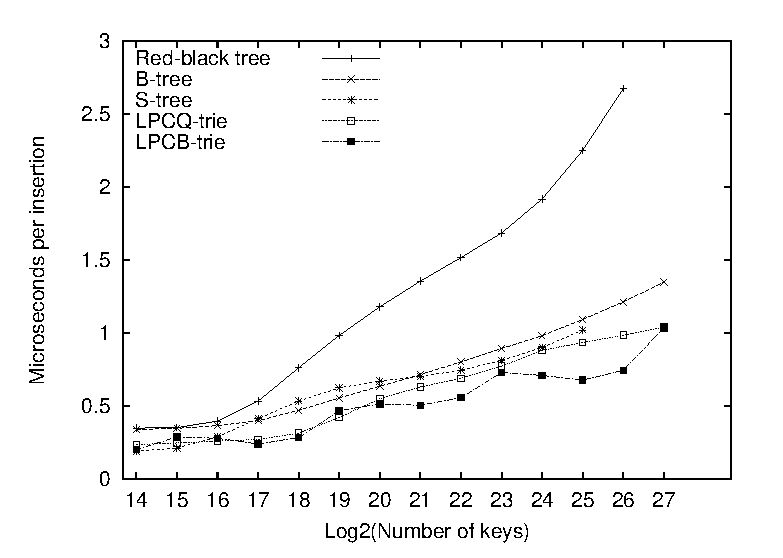
\includegraphics[width=0.8\textwidth]{plots/knuth_irandom_time.eps}\\
(a)\\
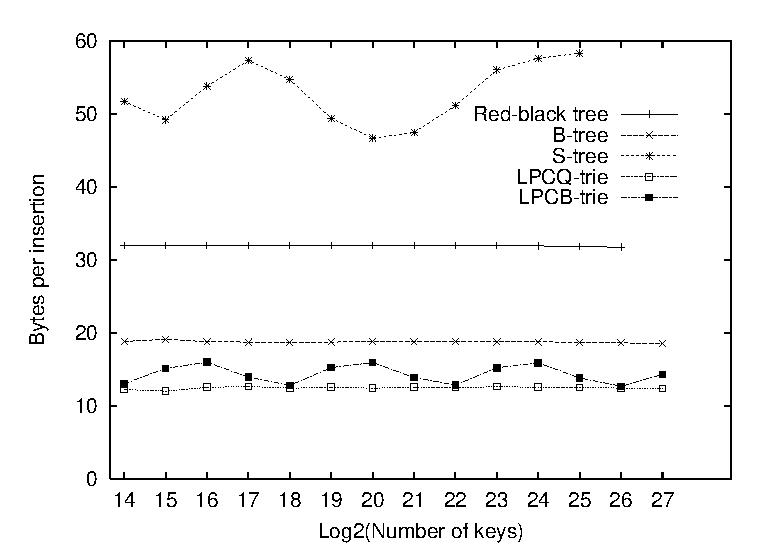
\includegraphics[width=0.8\textwidth]{plots/knuth_irandom_mem.eps}\\
(b)
\caption{This figure shows measurements gathered for uniform random 32-bit keys. 
(a) Shows the average time per insertion operation. The $LPCB$-trie performs best, and better than the comparison-based
structures at all input sizes, while the $LPCQ$-trie and $S$-tree also perform well. (b) Shows the space occupied by the data structures after a sequence
of insertions. The $LPCB$-trie and $LPCQ$-trie require the least space, and the $B$-tree is also competitive. We note that the $S$-tree
consistently requires a large amount of extra space compared to the other structures.
These results are discussed in Section \ref{random_results}}
\label{knuth_irandom_time_mem_fig}
\end{figure}

\begin{figure}
\center
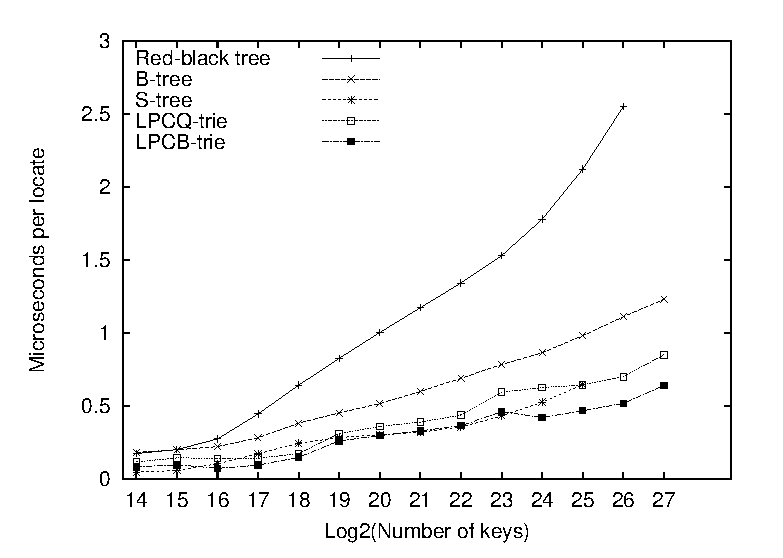
\includegraphics[width=0.8\textwidth]{plots/knuth_locate_time.eps}\\
(a)\\
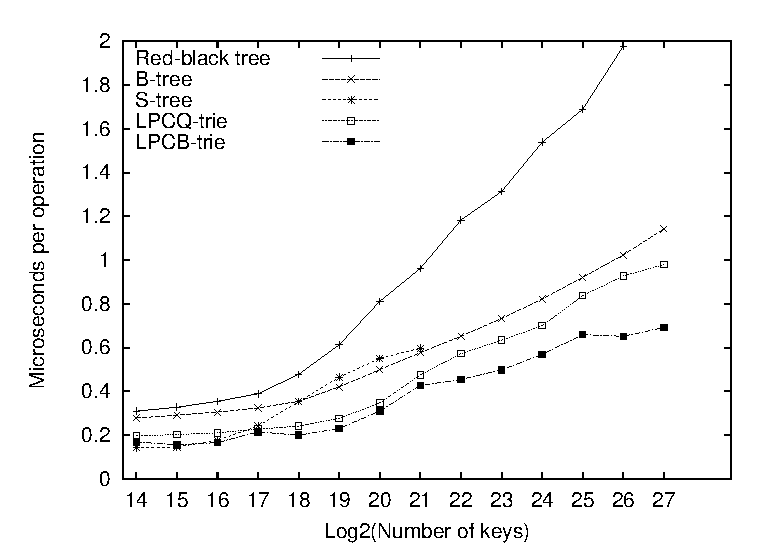
\includegraphics[width=0.8\textwidth]{plots/knuth_drandom_time.eps}\\
(b)
\caption{This figure shows measurements gathered for uniform random 32-bit keys.
(a) Shows the average time per locate operation
on the data structures as the number of keys in the structure increases. Note that results
are shown until the data structure occupies all of main memory. The $S$-tree performs very well, as does the $LPCB$-trie.
(b) Shows the average time per operation for a mixed sequence of equiprobable insertions and deletions. The deletions
are of keys that have already been inserted to the data structure.
These results are dicussed in Section \ref{random_results}.}
\label{knuth_locate_delete_time_fig}
\end{figure}

\comment{

MELODY STUFF REMOVED FOR NOW

\begin{figure}
\center
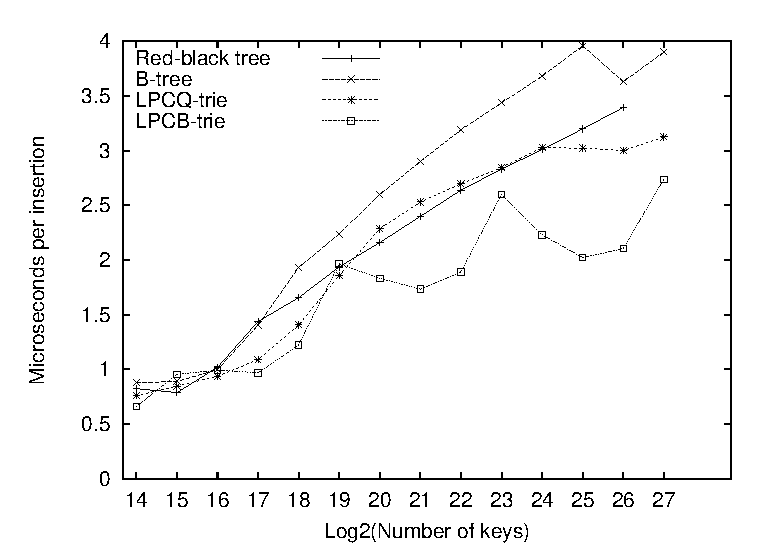
\includegraphics[width=0.8\textwidth]{plots/melody_irandom_time.eps}\\
(a)\\
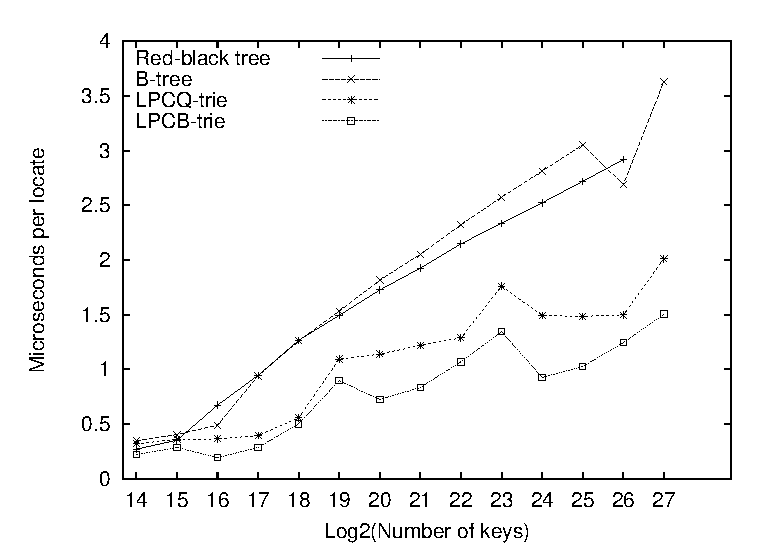
\includegraphics[width=0.8\textwidth]{plots/melody_locate_time.eps}\\
(b)
\caption{This figure shows measurements gathered on the \texttt{sparc} architecture for uniform random 32-bit keys. The $S$-tree
is not included on these plots because its implementation (CITE IMPLEMENTATION) is dependent on the endianness of the underlying
machine architecture, and it does not operate correctly on the \texttt{sparc} architecture.
(a) Shows the average time per insertion operation. We note that the these results differ substantially from the same data 
on the \texttt{x86} machine, shown in Figure \ref{knuth_irandom_time_mem_fig}(a). In general however, the $LPCB$-trie performs best,
especially for moderate to large inputs. (b) Shows the time per operation for a sequence of equiprobable insertions and deletions,
with the $LPCB$-trie once more out-performing the other data structures. The results are dicussed in Section \ref{random_results}}
\end{figure}

\begin{figure}
\center
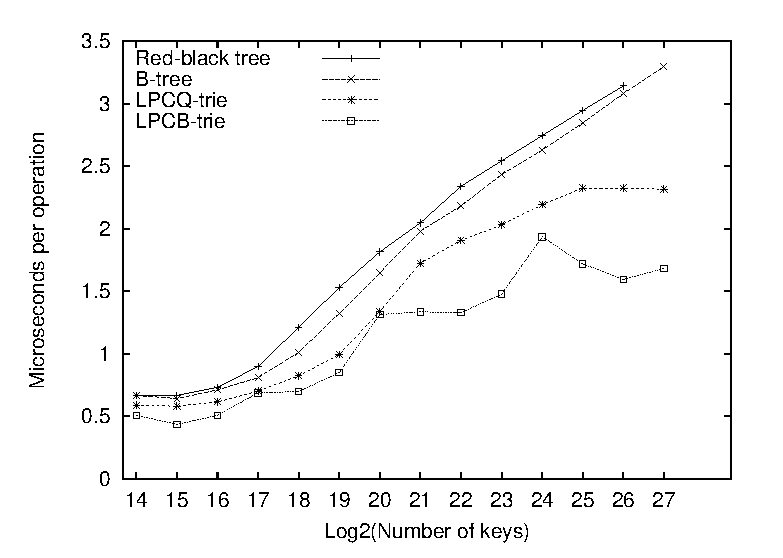
\includegraphics[width=0.8\textwidth]{plots/melody_drandom_time.eps}\\
\caption{32-bit: insert/delete mix (MELODY)}
\end{figure}

}

\begin{figure}
\center
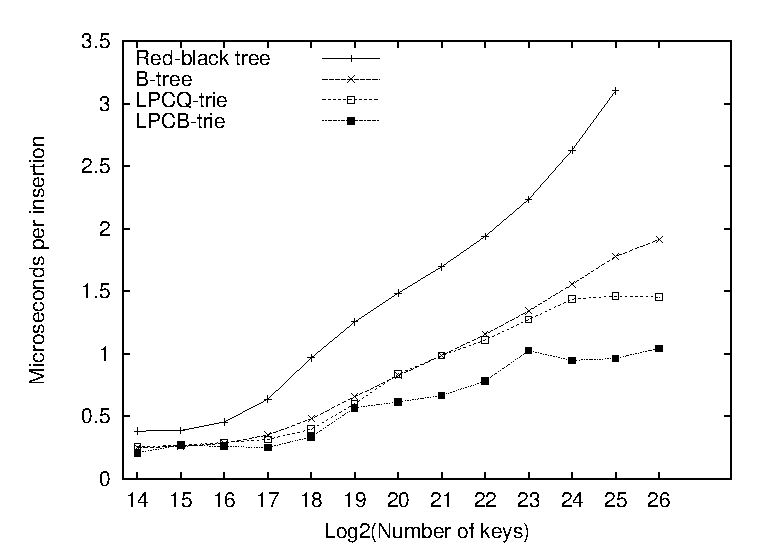
\includegraphics[width=0.8\textwidth]{plots/athena_irandom_time.eps}\\
(a)\\
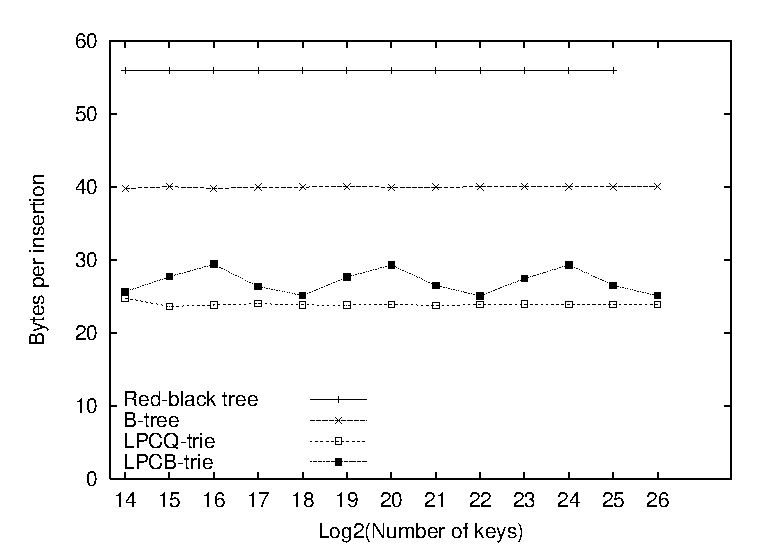
\includegraphics[width=0.8\textwidth]{plots/athena_irandom_mem.eps}\\
(b)\\
\caption{This figure shows measurements gathered for uniform random 64-bit keys. Note
that the $S$-tree does not appear in this figure because it is restricted to use with
32-bit keys. Results are shown until the data structures occupies all of main memory. 
(a) Shows the average time per insertion operation. The $LPCB$-trie performs best, and better than the comparison-based
structures at all input sizes, while the $LPCQ$-trie also performs well. (b) Shows the space occupied by the data structures after a sequence
of insertions. Again the $LPCQ$-trie requires the least space, followed by the $LPCB$-trie. As expected, both use approximately double what is
required in the 32-bit case, shown in Figure \ref{knuth_irandom_time_mem_fig}(b), as one expects. 
These results are discussed in Section \ref{random_results}.}
\label{athena_irandom_time_mem_fig}
\end{figure}

\begin{figure}
\center
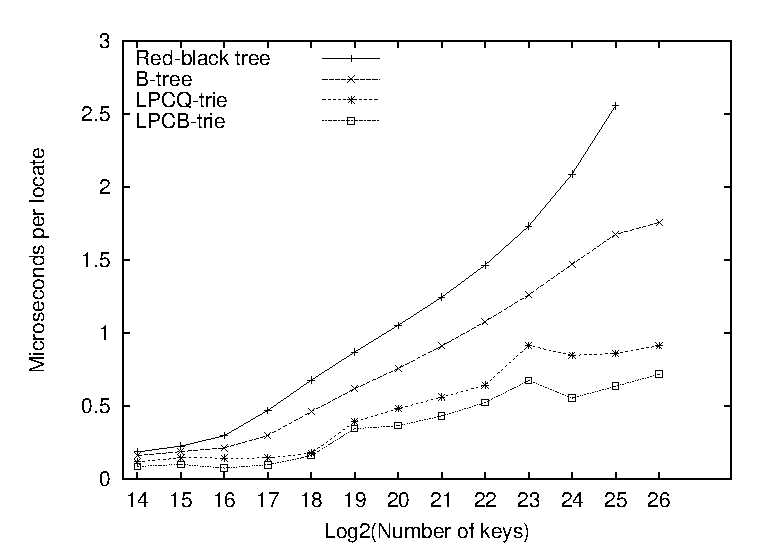
\includegraphics[width=0.8\textwidth]{plots/athena_locate_time.eps}\\
(a)\\
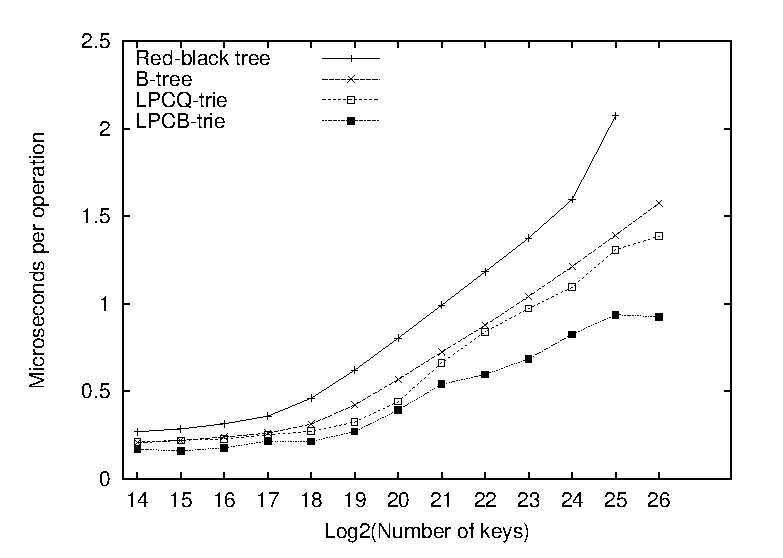
\includegraphics[width=0.8\textwidth]{plots/athena_drandom_time.eps}\\
(b)\\
\caption{
This figure shows measurements gathered for uniform random 64-bit keys. Note
that the $S$-tree does not appear in this figure because it is restricted to use with
32-bit keys. Results are shown until the data structures occupies all of main memory. 
(a) Shows the average time per locate operation. The $LPCB$-trie performs best, and better than the comparison-based
structures at all input sizes, while the $LPCQ$-trie also performs well. (b) Shows the time required for
a mixed sequence of equiprobable insertions and deletions. The deletions are of keys that are already present
in the data structures. These results are discussed in Section \ref{random_results}.}
\label{athena_locate_delete_time_fig}
\end{figure}

\subsection{Random Data}
\label{random_results}

Figure \ref{knuth_irandom_time_mem_fig}(a) shows the time per insertion for
the data structures over 32-bit uniform random keys. Note that the $S$-tree uses all available memory at
$2^{25}$ keys, while the red-black tree uses all available memory at $2^{26}$ keys.
Clearly the comparison-based structures are out-performed by the data structures tailored to integer keys.
In fact, the integer-specific data structures perform better than the comparison-based structures even for
the smallest inputs shown. Of the integer-specific structures, overall the $LPCB$-trie performs best. 

Figure \ref{knuth_irandom_time_mem_fig}(b) shows the memory consumption of the data structures for the insertions
of Figure \ref{knuth_irandom_time_mem_fig}(a). The $S$-tree is clearly a very memory hungry data structure, this,
combined with its restriction to 32-bit keys limits its practicality. After the $S$-tree the red-black tree requires the
second largest amount of memory per insertion\footnote{We say ``per insertion'' rather than ``per key'' because our we simply generate
a new uniform random key for each insertion, thus the keys are not distinct. Note also that for the data structure contain values associated with the keys.
In our experiments these values contain the same number of bits as the keys.}. Note that the data structures store a mapping
from a 32-bit key to a 32-bit value. The 32 bytes per insertion required by the red-black tree can be explained by considering the data
stored in each node of the tree: 4 bytes for each of: the key, the value, the left child pointer, the right child pointer, the parent pointer, 
and the node colour (due to alignment). Finally, there is an 8 byte overhead from the memory allocator.

The $B$-tree, which uses nodes consisting of arrays of keys of up 4KB in size, uses substantially less memory than the other comparison-based structure,
the red-black tree. The $LPCQ$-trie requires approximately 12 bytes per insertion --- the least memory of any the data structures. 
The $LPCB$-trie also has modest memory use, occupying between 12 and 16 bytes per insertion. This difference in memory consumption is likely a result
of the different approaches taken to bucket creation by the two data structures. The $LPCQ$-trie splits full buckets into exactly two new half-full buckets.
On the other hand, a full bucket in the $LPCB$-trie is burst into a potentially large number of new buckets. Naturally, when many small buckets are created the
space overhead per bucket is emphasized.

Figure \ref{knuth_locate_delete_time_fig}(a) shows the time per locate operation on the data structures, \texttt{locate}$(k)$ is the value associated
with the largest $k' \leq k$. Note that this operation is more general than can be answered efficiently with a hash table.
The integer-specific structures perform better than the comparison-based structures at all the input sizes shown in Figure \ref{knuth_locate_delete_time_fig}(a).
At the smallest input sizes the $S$-tree performs best. For the remainder of the input sizes, the $LPCB$-trie performs better. For $2^{25}$ insertions, the largest
data set before the $S$-tree exhausts main memory, the $LPCB$-trie's locate is approximately 30\% faster than the $S$-tree's. 
At $2^{27}$ insertions, the $LPCB$-trie's locate is approximately 30\% faster than the locate of its nearest competitor, the $LPCQ$-trie. 

Figure \ref{knuth_locate_delete_time_fig}(b) shows the time per operation for a mixed sequence of equiprobable insertions and deletions.
Unfortunately the only S-tree implementation available to us\footnote{Obtained
from \url{http://www.mpi-inf.mpg.de/~kettner/proj/veb/index.html}} had bugs in its delete operation causing it to
fail on inputs larger than $2^{21}$ operations. As with the results just described, the integer-specific data structures out-perform the
comparison-based structures, with the $LPCB$-trie peforming best in general.

We note that the $LPCQ$-trie and $LPCB$-trie use exactly the same implementations for their in-node data structures, bucket data structures as well as for the
level and path compressed tries. Their performance difference is a result of the fact that all operations in the $LPCQ$-trie begin with 
a predecessor search in the trie, which is slightly more complicated than a simple trie search. The other difference between the data structures
is that the $LPCQ$-trie splits rather than bursts buckets (as described in Section \ref{related_work}). Note also that due to the organization
of the $LPCB$-trie only key suffixes need be stored in buckets. In the $LPCQ$-trie, all keys in the same bucket do not share the same prefix, and so
it is not possible to simply store their suffixes. However, for simplicity, our current $LPCB$-trie implementation stores the entire keys in the buckets
and so this is not a factor in the performance difference observed in the experimental results just presented. Modifying the $LPCB$-trie
to store key suffixes will certainly reduce its space consumption even further, and it may also result in a performance improvement due to improved
spatial locality in its buckets.

The results for random 64-bit keys are shown in Figure \ref{athena_irandom_time_mem_fig} and Figure \ref{athena_locate_delete_time_fig}. The $S$-tree is excluded from
these results because it is tailored specifically for 32-bit keys, and
extending it efficiently to 64-bit keys requires an enormous amount of extra space.
For the remaining data structures the results for the 64-bit case are broadly similar to those observed in the 32-bit case. 
The $LPCB$-trie and $LPCQ$-trie perform better than the comparison-based data structures, with the B-tree performing substantially
better than the red-black tree.

In general, for both 32 and 64-bit uniform random keys, the $LPCB$-trie offers modest space usage and excellent performance
in time compared to the alternative data structures.


\subsection{Valgrind Data}
\label{valgrind_results_text}

\begin{figure}
\center
\begin{tabular}{cc}
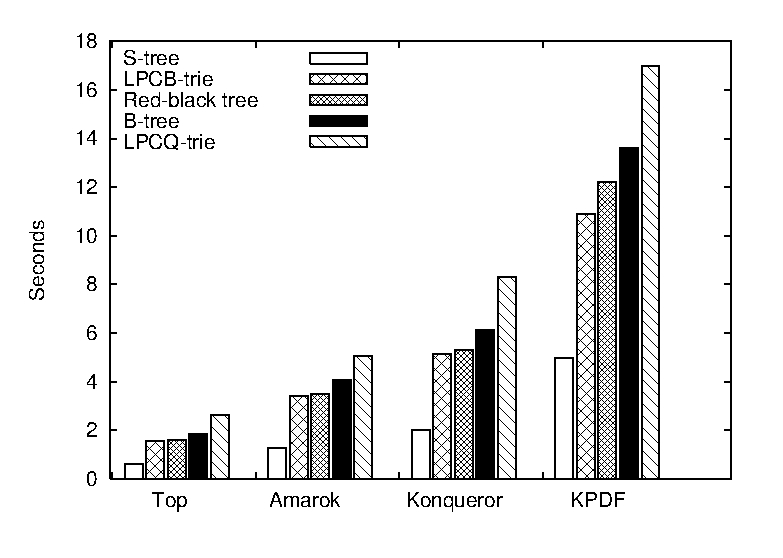
\includegraphics[width=0.45\textwidth]{plots/knuth_valgrind_time.eps} & 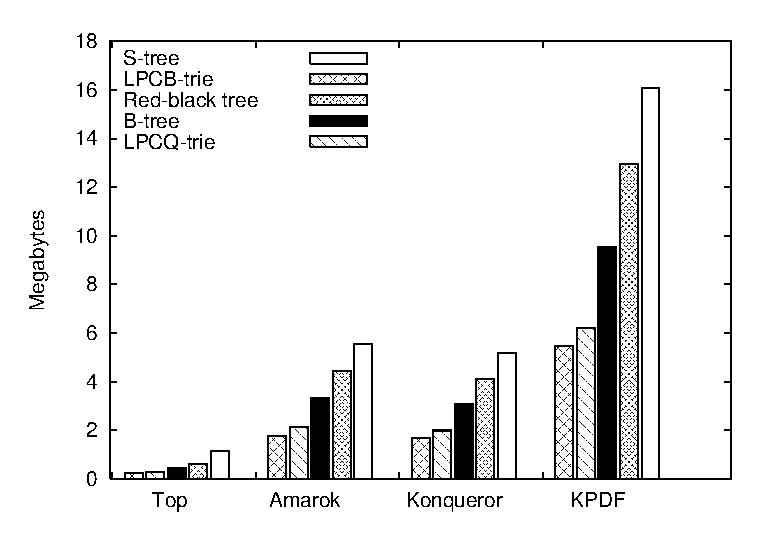
\includegraphics[width=0.45\textwidth]{plots/knuth_valgrind_mem.eps}\\
(a) & (b)\\
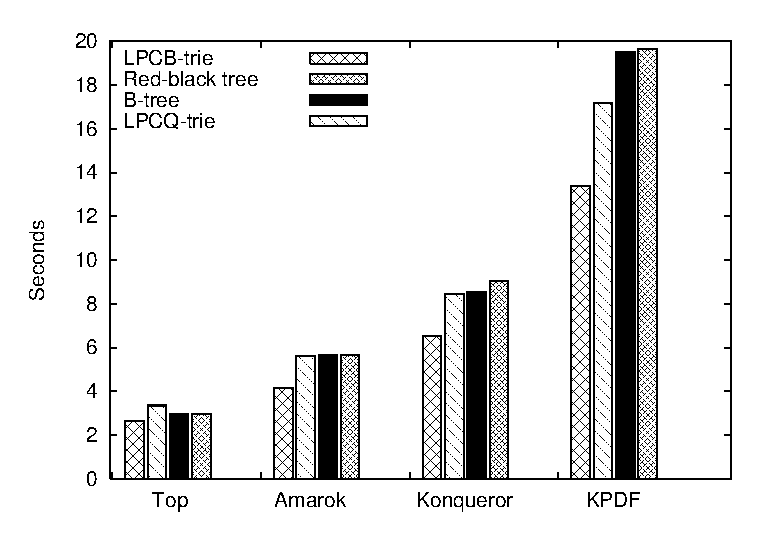
\includegraphics[width=0.45\textwidth]{plots/athena_valgrind_time.eps} & 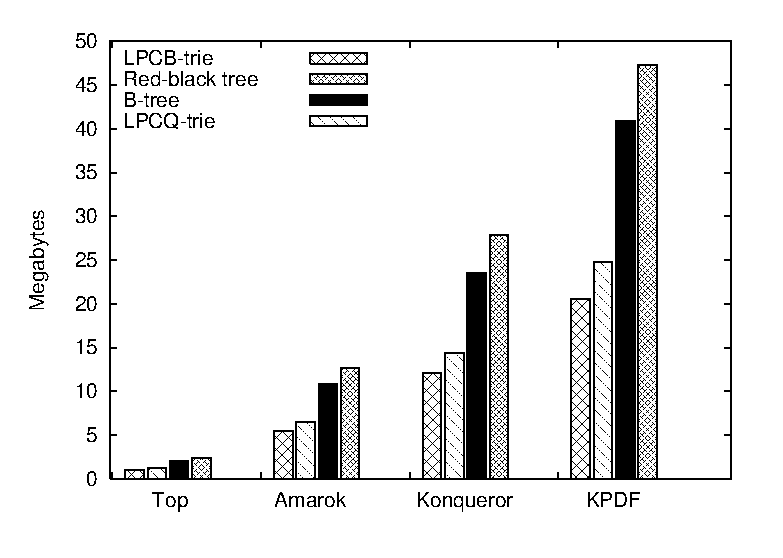
\includegraphics[width=0.45\textwidth]{plots/athena_valgrind_mem.eps}\\
(c) & (d)\\
\end{tabular}
\caption{This figure shows (a) the time, and (b) the space required by the
data structures to process the 32-bit Valgrind data sets. In (c) and (d) respectively
the time and space required to process the 64-bit Valgrind data sets are shown.
The results of (a) and (b) are gathered on the 32-bit machine, while the results
of (c) and (d) on the 64-bit machine. Note that the $S$-tree is not included in the 64-bit results
because it is restricted to 32-bit keys. The Valgrind data sets are described in Section \ref{exp_comparison}.
These results are discussed in Section \ref{valgrind_results_text}.}
\label{valgrind_results}
\end{figure}


\comment{

\begin{figure}
\center
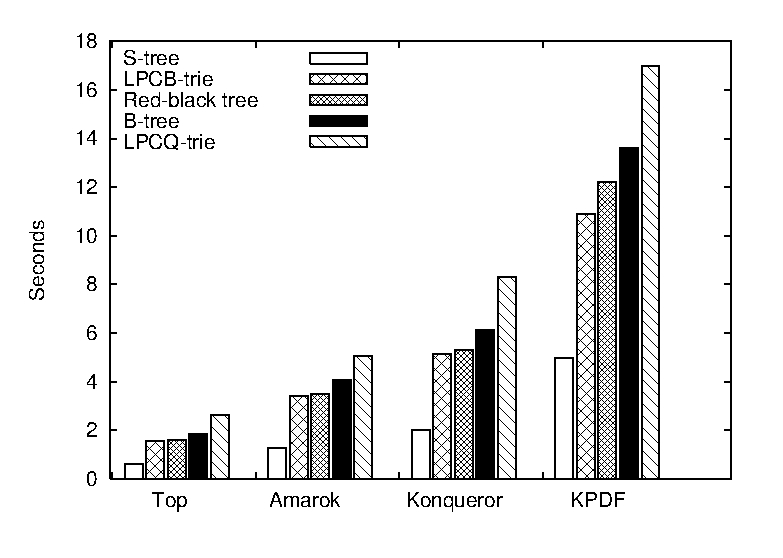
\includegraphics[width=0.8\textwidth]{plots/knuth_valgrind_time.eps}\\
(a)\\
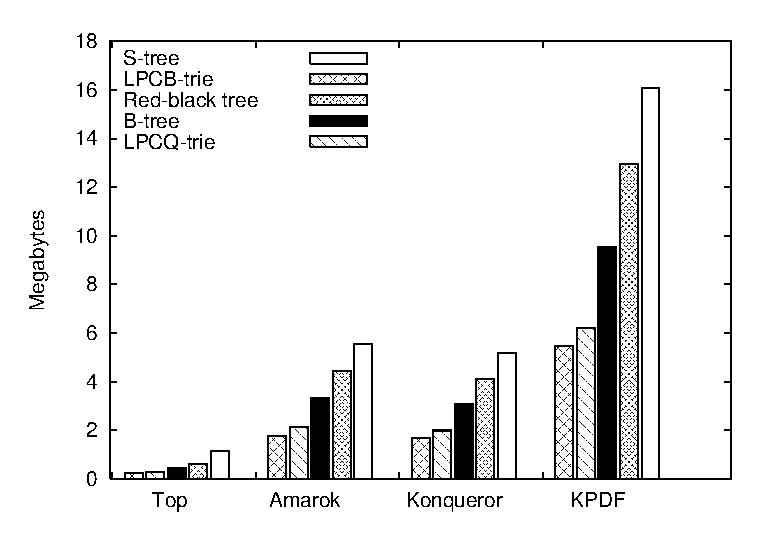
\includegraphics[width=0.8\textwidth]{plots/knuth_valgrind_mem.eps}\\
(b)
\caption{This figure shows the time, in (a) and space in (b) required by the
data structures to process the 32-bit Valgrind data-sets described in Section \ref{exp_comparison}.
These results are discussed in Section \ref{valgrind_results_text}}
\label{knuth_valgrind_results}
\end{figure}

\begin{figure}
\center
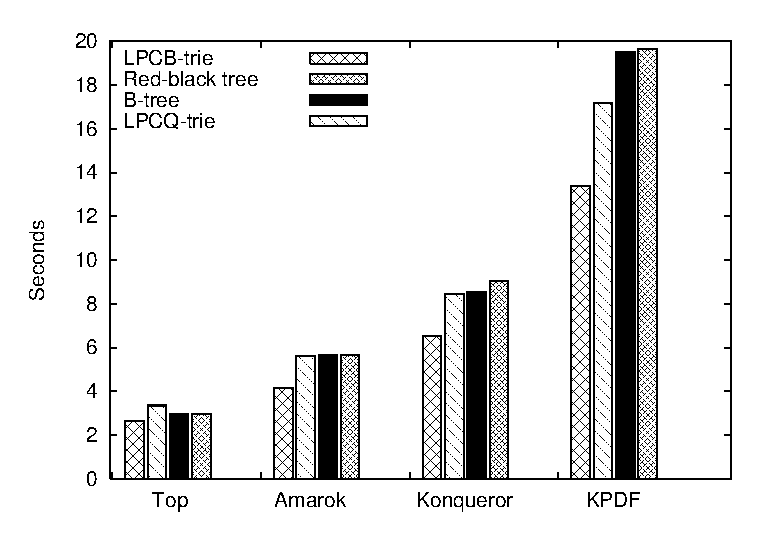
\includegraphics[width=0.8\textwidth]{plots/athena_valgrind_time.eps}\\
(a)\\
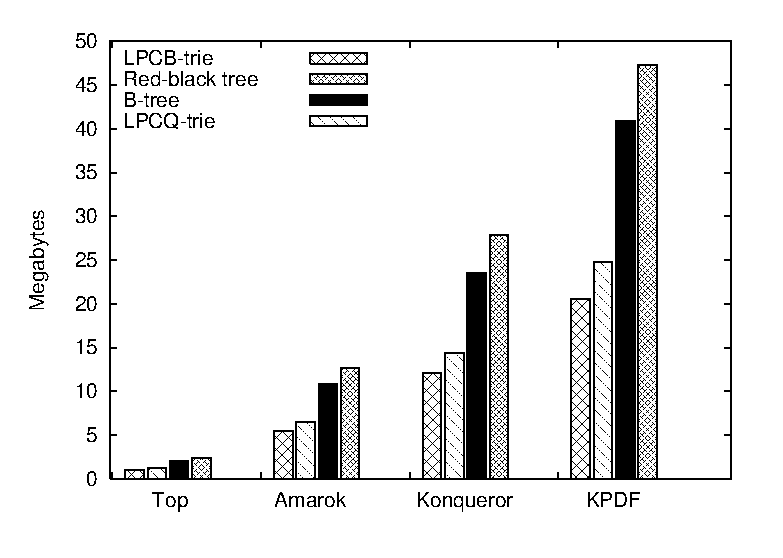
\includegraphics[width=0.8\textwidth]{plots/athena_valgrind_mem.eps}\\
(b)
\caption{This figure shows the time, in (a) and space in (b) required by the
data structures to process the 64-bit Valgrind data-sets described in Section \ref{exp_comparison}.
Note that the $S$-tree is not shown because it is restricted to 32-bit keys.
These results are discussed in Section \ref{valgrind_results_text}}
\label{athena_valgrind_results}
\end{figure}
}

Figure \ref{valgrind_results}(a) shows the time for processing 32-bit Valgrind data sets of various programs (these data sets
are described in Section \ref{exp_comparison}). On these data sets, the $S$-tree is clearly the most efficient data structure in time, followed by
the $LPCB$-trie. It is notable that the $B$-tree performs worse than the red-black tree on these data sets. Moreover, the $LPCB$-trie performs
only slightly better than the red-black tree. This margin should be compared with the margin observed between the $LPCB$-trie and red-black
tree over the uniform random data, up to about $2^{19}$ keys (since as described in Section \ref{exp_comparison}, the largest Valgrind data
set contains fewer than 500,000 distinct keys). It is notable that the $LPCQ$-trie performs the worst on these Valgrind data sets. 

Figure \ref{valgrind_results}(b)
shows the memory consumed by the data structures in processing the data sets. For all the data sets, the $LPCB$-trie
requires the least memory of any of the data structures. Once again, the $S$-tree is seen to be especially inefficient in space
compared to the other data structures.

Figure \ref{valgrind_results}(c) shows the time for processing the Valgrind data sets in the 64-bit case. The $S$-tree
is excluded because it cannot operate on 64-bit keys. The $LPCB$-trie is the most efficient data structure. 
As Figure \ref{valgrind_results}(d) shows, the $LPCB$-trie is also the most space efficient data structure on the data sets. 

On the 32-bit data sets, the $S$-tree performs better than the $LPCB$-trie, however, it requires more than twice as much memory.
On the 64-bit data sets, the $LPCB$-trie is the best performing data structure, as well as requiring the least space of
any data structure.

\subsection{Genome Data}

\begin{figure}
\begin{tabular}{cc}
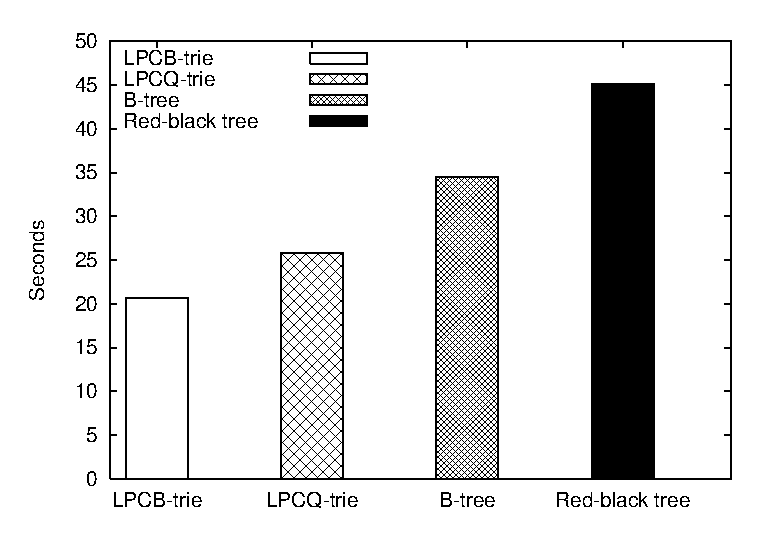
\includegraphics[width=0.45\textwidth]{plots/athena_36_genome_time.eps} & 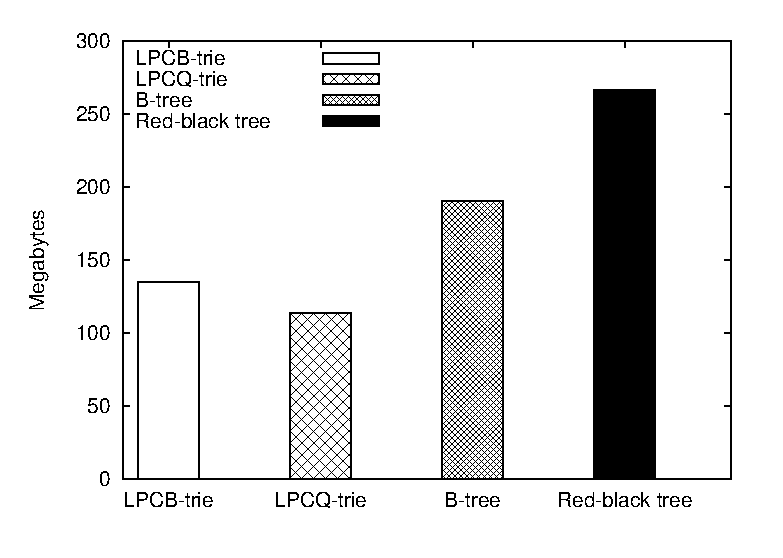
\includegraphics[width=0.45\textwidth]{plots/athena_36_genome_mem.eps}\\
(a) & (b)
\end{tabular}
\caption{This figure shows results for processing the Genome data set (described in Section \ref{exp_comparison}). 
These results were gathered on the 64-bit machine. The keys are 36-bit integers. In (a), the time to insert and then search
for all the keys of the data set is shown. While (b) shows the space required by each data structure.}
\label{athena_genome_36_fig}
\end{figure}


The final experimental results we present are for the genome data set, described in Section \ref{exp_comparison}.
Figure \ref{athena_genome_36_fig}(a) shows the time taken by the data structures to insert all the keys of the
genome set, and then search for them in turn. Again, the $S$-tree is not shown because it is restricted to
32-bit keys. The $LPCB$-trie is approximately $40\%$ faster than the $B$-tree, the more efficient of the comparison-based structures, and
approximately $20\%$ faster than the $LPCQ$-trie.
As Figure \ref{athena_genome_36_fig}(b) shows, the $LPCB$-trie's memory usage is approximately half that of the red-black tree
and approximately $70\%$ of the $B$-tree's. In this case, the least memory is used by the $LPCQ$-trie, requiring
approximately $20\%$ less memory than the $LPCB$-trie.



\comment{

MELODY STUFF REMOVED FOR NOW

\begin{figure}
\center
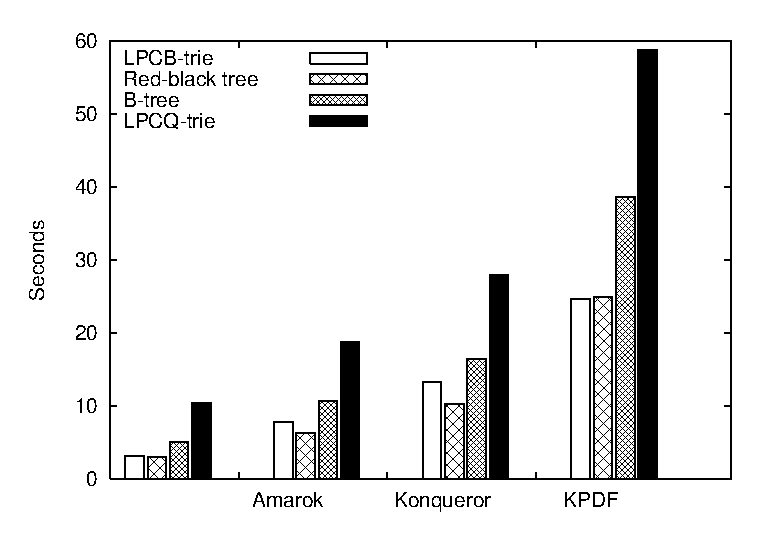
\includegraphics[width=0.8\textwidth]{plots/melody_valgrind_time.eps}\\
(a)\\
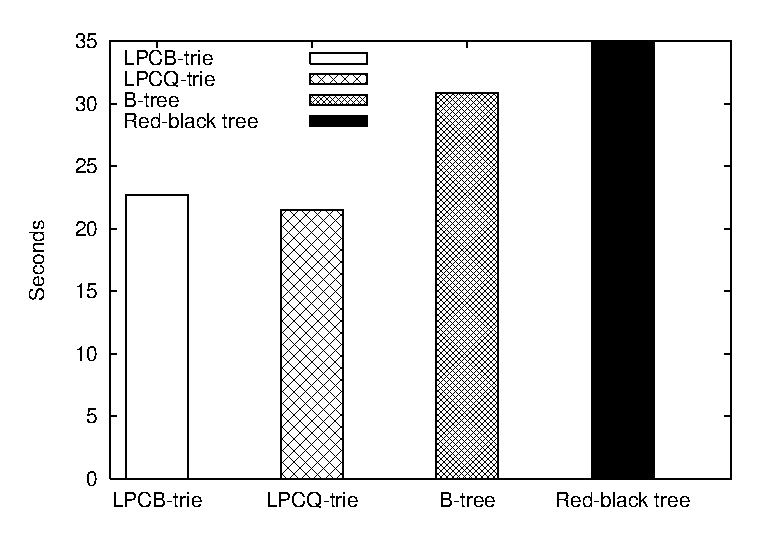
\includegraphics[width=0.8\textwidth]{plots/melody_genome_time.eps}\\
(b)
\caption{32-bit: (a) valgrind trace time (b) genome time (SPARC)}
\end{figure}

}


\comment{

\begin{figure}
\begin{tabular}{cc}
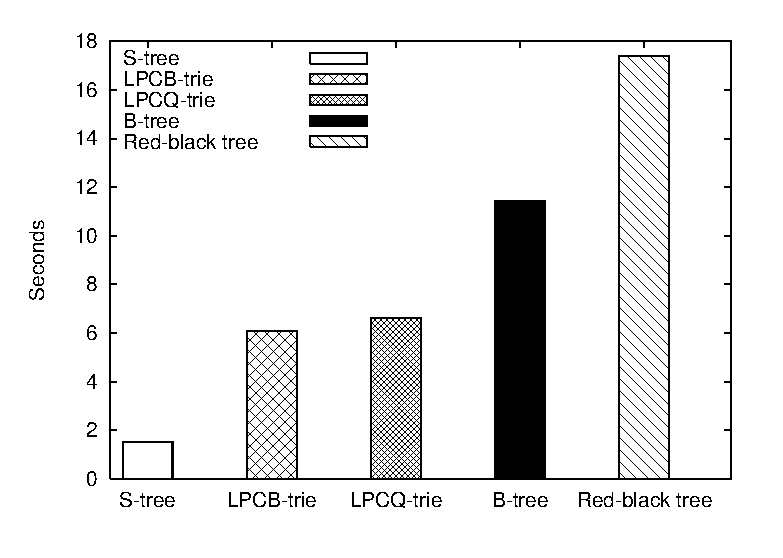
\includegraphics[width=0.45\textwidth]{plots/knuth_genome_time.eps} & 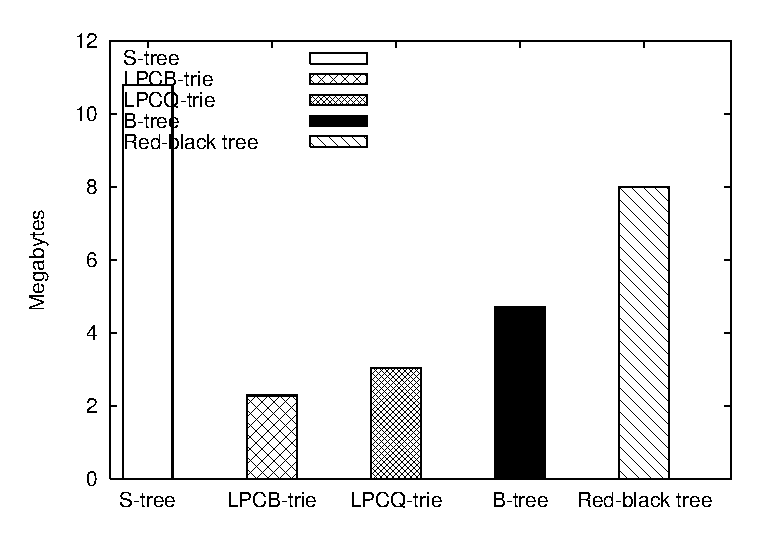
\includegraphics[width=0.45\textwidth]{plots/knuth_genome_mem.eps}\\
(a) & (b)
\end{tabular}
\caption{32-bit: (a) genome processing time (b) space used}
\end{figure}

}


\section{Conclusion and Future Work}

This paper has provided an experimental comparison of efficient data structures operating over 32 and 64-bit integer
keys. In particular we have shown that extending burst tries to an ordered data structure for integer keys 
provides a data structure that is very efficient in both time and space.

In comparisons using uniform random data with
red-black trees and $B$-trees we have shown that our level and path compressed variant of burst tries, $LPCB$-tries, 
provide all operations more efficiently in both time and space. We have also compared our $LPCB$-trie to Dementiev \textit{et al.}'s \citeyear{Dementiev+04}
$S$-tree data structure based on stratified trees, and found that while Dementiev \textit{et al.}'s data structure is competitive
in time, it requires far more memory than an $LPCB$-trie and is less general, being restricted to 32-bit keys.
We have also compared $LPCB$-trie to $Q$-tries, a data structure based on Korda and Raman's \citeyear{KordaRaman99} modification of Willard's \textit{q}-fast tries \citeyear{Willard84}.
We carefully engineered an implementation of $LPCQ$-tries, using the same bucket and node data structures as our burst trie as well as incorporating level compression, and found
that they are generally slightly less efficient in time than $LPCB$-tries. The $LPCQ$-tries requires slightly less space however. On the uniform random data, we found the $LPCB$-trie
to require 12 and 16 bytes per insertion, whereas the $LPCQ$-trie required approximately 12 bytes per insertion.

We have also presented results for an application of dynamic, ordered integer data structures in Valgrind where the keys are 32 and 64-bit integers.
Our results show that in the 32-bit case only the $S$-tree data structure operates faster than the $LPCB$-trie, but the $S$-tree requires almost
twice as much space as the $LPCB$-trie. In the 64-bit case, the $LPCB$-trie requires less space and operates more rapidly
than any of the alternative data structures. We also provided experimental results over a data set derived from a Genome data set, where the
keys are 36-bit integers. In this case, the $LPCB$-trie operated substantially faster and required less space than the alternative comparison-based structures.

One advantage of a burst trie over a $Q$-trie is that because of a burst trie's organisation, it need only store key suffixes in buckets, improving space usage as
well as spatial locality. The experimental results for the implementation of the $LPCB$-trie presented in this paper in fact stores entire keys -- and not just their suffixes --
in buckets. We plan to left this restriction in the near future and investigate the storage of only key suffixes in buckets. This will certainly offer 
improvements in space, and may also result in better performance of the $LPCB$-trie due to improved spatial locality in its buckets.

This paper demonstrates, through the application $LPCB$-tries in Valgrind together with the results presented over the Genome and random data, 
that $LPCB$-tries should be considered as one of the many alternative data structures for applications requiring a general purpose dynamic ordered data structure 
over keys such as integers or floating point numbers.

\ack{The authors thank Julian Seward for useful discussions and his patient assistance with Valgrind. We also thank Robert Crosbie
for many useful comments.
This paper incorporates work previously published in ``Comparing Integer Data Structures for 32 and 64 Bit Keys'', N. Nash
and D. Gregg, In \textit{Proceedings of the 8th International Workshop on Experimental Algorithms} (WEA), Provincetown, Cape Cod, MA, 
USA, June 2008. The authors thank the WEA referees for their helpful comments.}

\bibliographystyle{acmtrans}
\bibliography{paper}
\begin{received}
\end{received}

\end{document}


